% !TEX program = xelatex
% 2026 年高教社杯全国大学生数学建模竞赛 A 题
% 药材的烘干问题 —— 论文全文（单文件完整版）
% 由 摘要与总论.tex、问题一.tex、问题二三四.tex 合并而成

\documentclass[12pt,a4paper,fontset=none]{ctexart}

% 中文字体：显式指定，避免依赖系统字体集探测
\usepackage{xeCJK}
\setmainfont{Times New Roman}
\setsansfont{Arial}
\setmonofont{Menlo}
\setCJKmainfont{Songti SC}
\setCJKsansfont{Heiti SC}
\setCJKmonofont{Songti SC}

\usepackage{amsmath,amssymb,bm}
\usepackage{booktabs}
\usepackage{multirow}
\usepackage{array}
\usepackage{geometry}
\usepackage{caption}
\usepackage{graphicx}

\geometry{left=2.7cm,right=2.7cm,top=2.6cm,bottom=2.6cm}
\captionsetup{font=small,labelsep=quad}
\linespread{1.32}
\allowdisplaybreaks

\begin{document}


\begin{center}
  {\zihao{3}\bfseries 药材烘干过程的传热传质建模与数值仿真}
\end{center}

\vspace{0.5em}
\begin{center}
  {\zihao{4}\bfseries 摘\quad 要}
\end{center}

\noindent
中药材烘干是决定成品品质的关键工序。热风烘干包含预热平衡与恒温干燥两个阶段，
工艺参数选取不当会造成干燥效率低、能耗高、品质不稳定。本文针对圆柱形药材，
建立了径向耦合传热传质数学模型，并对四个问题给出定量解答。

\textbf{针对问题一}，考虑药材长径比达 6.25、端面仅占侧面 8\%，
将其简化为无限长圆柱的一维径向轴对称问题。由附录 2 的物性算得热扩散率
$\alpha=1.689\times10^{-7}$\,m$^2$/s 与水分扩散系数
$D(C_0)=4.938\times10^{-9}$\,m$^2$/s 相差 34 倍，
1800\,s 内热扩散长度 17.4\,mm 已接近半径而水分扩散长度仅 2.98\,mm，
由此判断该阶段以达热平衡为主。关键的结构性质是：$D$ 只依赖 $C$ 不含 $T$、
其余物性为常数，故\textbf{热方程与水分方程完全解耦}，可分别独立求解。
采用节点中心有限体积法配合后向 Euler 与 Picard 迭代求解，水分守恒残差为
$6.8\times10^{-14}$（机器精度）。结果表明：1800\,s 内药材中心含水率始终保持
2.5500\,kg/kg，而表面已降至 1.5103，水分变化局限在最外侧约 $3\sim5$\,mm；
温度则在整个截面上重新分布，中心 33.5765\,$^\circ$C、表面 36.7863\,$^\circ$C，
径向温差 3.21\,$^\circ$C。

\textbf{针对问题二}，附录 3 给出 $\rho$、$c_p$、$k$ 随 $C$ 变化、
$D$ 随 $C$ 与 $T$ 变化的经验式，两方程由解耦转为强耦合，必须联立迭代。
由附件 1 末段 1\,h 的平均值（49.9989\,$^\circ$C、0.04999\,kg/kg）
确定恒温干燥段工况为 50\,$^\circ$C 与 0.05\,kg/kg。结果表明药材在约 2.5\,h
内基本达到烘房温度（3\,h 时径向温差仅 0.12\,$^\circ$C），含水率则依
"由表及里"的次序下降：0.5\,h 时中心未变而表面已降至 1.6233，
3\,h 时中心 1.9721、表面 1.0655，全过程始终由内部扩散控制。

\textbf{针对问题三}，烘干判据"各处含水率低于 0.15\,kg/kg"等价于中心处达标，
即 $t_{\mathrm{dry}}=\min\{t\mid C(0,t)<0.15\}$。求得
\textbf{烘干时长 61.02\,h（2.543 天）}，落在题面所述 $2\sim3$ 天区间内；
其中 36\,h 之后中心由 0.1941 缓慢逼近 0.15 竟耗时约 25\,h，
占总时长的 41\%，是工程上最不经济的阶段。

\textbf{针对问题四}，附件 2 显示半径由 2.000\,cm 收缩至 1.198\,cm，
且收缩高度前置（50\% 的收缩在 2.5\,h 内完成，99\% 在 22\,h 内完成），
而含水率的缓慢下降持续到 50\,h 之后，说明二者不存在简单对应关系，
故直接采用实测 $R(t)$。引入贴体坐标 $\xi=r/R(t)$ 将动边界化为固定区域，
方程相应增加对流项 $\xi R\dot R\,\partial C/\partial\xi$；
$R(t)$ 用保单调的三次 Hermite 插值以避免 $\dot R$ 跳变。
求得\textbf{烘干时长 50.31\,h（2.096 天）}，比不考虑收缩时缩短 17.6\%；
作为对照，同一物性下固定半径的烘干时长为 5.71 天，可见
\textbf{忽视收缩会将烘干时长高估约 1.7 倍}。

\textbf{本文的特色}在于四点。

一是\textbf{完整的数据预处理论证}。实测数据是否平滑、是否换用高阶插值、
能否用差分估计变化率，都是会改变四位小数结果的选择。本文对附件 1 作了
噪声诊断（残差标准差 $0.116\,^\circ$C、高频交替型、无异常点、无缺失），
并给出量化结论：\textbf{不应对附件 1 作平滑}——药材热时间常数 2368\,s 是
噪声周期的 20--40 倍，平滑只会削去被过滤掉的成分，而三维对比实验表明
含水率场几乎不受预处理方式影响（四位小数下至多 $0.2\%$ 的格子变化，
问题二表 4 的 30 个数字完全不变），温度场的差异则仅有
$0.002\sim0.027\,^\circ$C，小于噪声本身不可消除的 $0.02\,^\circ$C 涨落。
据此明确声明温度结果的有效位为 3 位，并说明附件 1 \textbf{在原理上不能用
于反求 $h$、$h_m$}（只有边界激励、没有药材侧响应，参数不可辨识）。附件 2
因需要测点间连续的收缩速率，采用保单调三次 Hermite 插值。

二是\textbf{严格区分了问题一中热质解耦与问题二中热质耦合的结构性差异}，
并对题面未给出的闭合关系（传质边界条件的密度口径、汽化潜热）作了定量讨论，
依据湿球温度下限判断出题面隐含忽略汽化潜热。

三是\textbf{完成了参数灵敏度分析与基于实测数据的守恒性检验}。前者表明过程
由内部水分扩散控制：$D$ 变化 $\pm20\%$ 使烘干时长在 $51.9\sim74.5$\,h 之间
摆动，而表面换热系数 $h$ 的影响仅 $\pm0.05\%$、传质系数 $h_m$ 仅
$\pm2\sim3\%$——即使附录给出的 $h$、$h_m$ 存在成倍误差，结论也基本不变；
后者用附件 2 的实测半径检验干物质守恒，发现并如实报告了题面两组给定数据
之间存在的不自洽（问题三 $+116\%$、问题四 $-11\%$）。

四是\textbf{全部结果通过了守恒性、网格与时间步收敛性、独立求解器交叉验证
以及水分方程口径的三方案对照}。四个问题算得的烘干时长均与题面给出的
2--3 天量级自洽。

\vspace{1em}
\noindent\textbf{关键词}：\ 热风干燥；耦合传热传质；圆柱坐标；有限体积法；
动边界；收缩；汽化潜热；\textbf{数据预处理}；灵敏度分析

\newpage

\section{问题重述}

\subsection{问题背景}

干燥是决定中药材成品品质的关键工序之一，热风烘干是常见方式，
包括预热平衡与恒温干燥两个阶段。工艺参数选取不当会导致干燥效率低、
能耗高、成品品质不稳定；传统试验优化成本高、周期长，
故需借助数理分析与数值仿真获得干燥规律。

\subsection{问题提出}

某圆柱形中药材长 25\,cm、半径 2\,cm，初始温度 28\,$^\circ$C、
初始干基含水率 2.55\,kg/kg。烘房空气的温度与水分浓度见附件 1，
附录 2 给出问题一的物性参数，附录 3、4 分别给出问题二/三与问题四的
经验公式，附件 2 给出烘干过程中药材半径的变化。需要解决：

\begin{enumerate}
  \item 建立预热平衡阶段药材温度与水分浓度变化的数学模型，
        给出 1800\,s 内按指定时空格点采样的结果；
  \item 建立整个烘干过程（预热平衡 $+$ 恒温干燥）的数学模型，
        给出 3\,h 内的结果；
  \item 按"各处含水率低于 0.15\,kg/kg"的要求确定烘干所需时间；
  \item 考虑药材因失水发生的尺寸变化，重新确定烘干时长。
\end{enumerate}

\section{问题分析}

四个问题本质上求解同一个物理过程的不同层面：

\begin{table}[htbp]
  \centering
  \caption{四个问题的差异}
  \label{tab:overview}
  \small
  \begin{tabular}{llll}
    \toprule
    问题 & 物性来源 & 时间跨度 & 结构性特点 \\
    \midrule
    一 & 附录 2（恒定）        & 30 min  & 热、质方程解耦 \\
    二 & 附录 3（随 $C$、$T$） & 2--3 天 & 强耦合，需联立迭代 \\
    三 & 附录 3                & 2--3 天 & 反求达标时刻 \\
    四 & 附录 4（随 $C$、$T$） & 2--3 天 & 动边界，需坐标变换 \\
    \bottomrule
  \end{tabular}
\end{table}

问题的物理内核是\emph{含湿多孔介质内的耦合传热传质}：热量由表面向内部传导，
水分由内部向表面迁移并在表面被流动的空气带走，两者通过随含水率、
温度变化的物性相互影响。

三个量级分析决定了建模方向。其一，长径比与端面占比说明可退化为
一维径向问题；其二，热扩散率与水分扩散系数相差数十倍，
说明温度与水分的时间尺度不同，预热阶段以达热平衡为主；其三，
两个 Biot 数均处于中值区间，说明不能作集总参数近似，
必须给出沿半径的分布。

\section{模型假设}

\begin{enumerate}
  \item[(A1)] 药材均质、各向同性，孔隙水与固体骨架局部热平衡；
  \item[(A2)] 忽略轴向输运，问题简化为一维径向轴对称；
  \item[(A3)] 无内热源、忽略辐射，仅考虑表面对流换热与对流传质；
  \item[(A4)] 问题一至三不考虑尺寸变化，问题四按附件 2 的实测半径收缩；
  \item[(A5)] 物性按各问对应附录取值；问题一中 $\rho$、$c_p$、$k$ 为常数
        且 $D=D(C)$，问题二起 $D=D(C,T)$、$\rho,c_p,k$ 随 $C$ 变化；
  \item[(A6)] 对流换热系数与对流传质系数题面未给出，统一沿用附录 2 的
        $h=25$\,W/(m$^2\cdot$K)、$h_m=8\times10^{-7}$\,m/s；
  \item[(A7)] 忽略汽化潜热对能量平衡的贡献。若按同一密度口径计入，
        表面温度会被压至 $6.1\,^\circ$C，低于由空气状态算得的湿球温度
        $34.7\,^\circ$C，与热力学第二定律矛盾，故判定题面所给参数体系
        隐含该项可略；
  \item[(A8)] 水分的输运用 Fick 型扩散描述，表面传质用第三类边界条件描述。
  \item[(A9)] 附件 1 的烘房温湿度实测序列\textbf{不作平滑、不作差分、
        不剔除观测点}，直接以 60\,s 分段线性插值作为边界条件
        $T_\infty(t)$、$C_\infty(t)$，依据与量化影响见
        第 \ref{sec:preproc} 节；
  \item[(A10)] 附件 2 的半径序列改用保单调三次 Hermite 插值（PCHIP），
        以其解析导数 $\dot R$ 作为收缩速率，理由见第 \ref{sec:preproc} 节。
\end{enumerate}

\newpage
\section{符号说明}

\begin{center}
\begin{minipage}{\textwidth}
  \centering
  \small
  \textbf{主要符号}\\[4pt]
  \begin{tabular}{cll}
    \toprule
    符号 & 含义 & 单位 \\
    \midrule
    $r,\ t$            & 径向坐标、时间              & m, s \\
    $T,\ C$            & 药材温度、干基含水率        & $^\circ$C, kg/kg \\
    $R,\ L$            & 药材半径、长度              & m \\
    $\xi$              & 贴体坐标 $\xi=r/R(t)$       & --- \\
    $T_\infty,C_\infty$ & 烘房空气温度、水分浓度     & $^\circ$C, kg/kg \\
    $\rho,\ c_p,\ k$   & 密度、比热容、热传导系数    & kg/m$^3$, J/(kg$\cdot$K), W/(m$\cdot$K) \\
    $D$                & 水分扩散系数                & m$^2$/s \\
    $h,\ h_m$          & 对流换热、传质系数          & W/(m$^2\cdot$K), m/s \\
    $\alpha$           & 热扩散率                    & m$^2$/s \\
    $Bi,\ Bi_m$        & 传热、传质 Biot 数          & --- \\
    $t_{\mathrm{dry}}$ & 烘干时长                    & s \\
    \bottomrule
  \end{tabular}
\end{minipage}
\end{center}




\section{数据预处理}
\label{sec:preproc}

本题只给两个数据附件：附件 1 是烘房空气的温湿度时序，在模型中充当
\emph{边界激励}；附件 2 是药材半径的时序，在问题四中充当\emph{动边界}。
二者的物理角色不同，对预处理的要求也完全不同。本节先给出数据质量诊断，
再逐项说明为什么\textbf{附件 1 不作任何平滑、不作高阶插值、不作差分，
而附件 2 必须作保单调插值}，并量化这些选择对最终结果的影响。
全部结论均由独立复算给出，可复现。

\subsection{附件 1 的数据质量诊断}

附件 1 共 241 个采样点，间隔 60\,s，覆盖 $0\sim14400$\,s。用无相位滞后的
局部二次多项式分离趋势后，残差统计如表 \ref{tab:noise}。

\begin{table}[htbp]
  \centering
  \caption{附件 1 实测序列的噪声诊断}
  \label{tab:noise}
  \small
  \begin{tabular}{lccccc}
    \toprule
    量 & 趋势范围 & 残差标准差 & 最大残差 & 滞后 1 自相关 & 占全变幅 \\
    \midrule
    烘房温度 $T_\infty$ & $28.00\to50.00\,^\circ$C & $0.116\,^\circ$C
      & $0.27\,^\circ$C & $-0.31$ & $0.52\%$ \\
    水分浓度 $C_\infty$ & $0.0196\to0.0500$ & $1.1\times10^{-4}$
      & $2.8\times10^{-4}$ & $-0.40$ & $0.38\%$ \\
    \bottomrule
  \end{tabular}
\end{table}

三个特征决定了后文的处理方式。其一，残差的滞后 1 自相关为负，
说明它是\textbf{高频交替型}抖动——来自传感器噪声或烘房控温的往复调节，
而不是真实的物理起伏。其二，幅度很小，最大残差仅为残差标准差的 2.3 倍，
\emph{不存在需要判别与剔除的异常点}，强行剔除反而会削掉真实的控制波动。
其三，数据\textbf{无缺失、无负值，温度全局最低点即为 $t=0$ 的
$28.0000\,^\circ$C}，未出现低于初值的非物理值，水分浓度亦恒为正。
因此附件 1 \emph{不需要}通常意义上的清洗（实测序列与噪声诊断见
图 \ref{fig:air}）。

\begin{figure}[htbp]
  \centering
  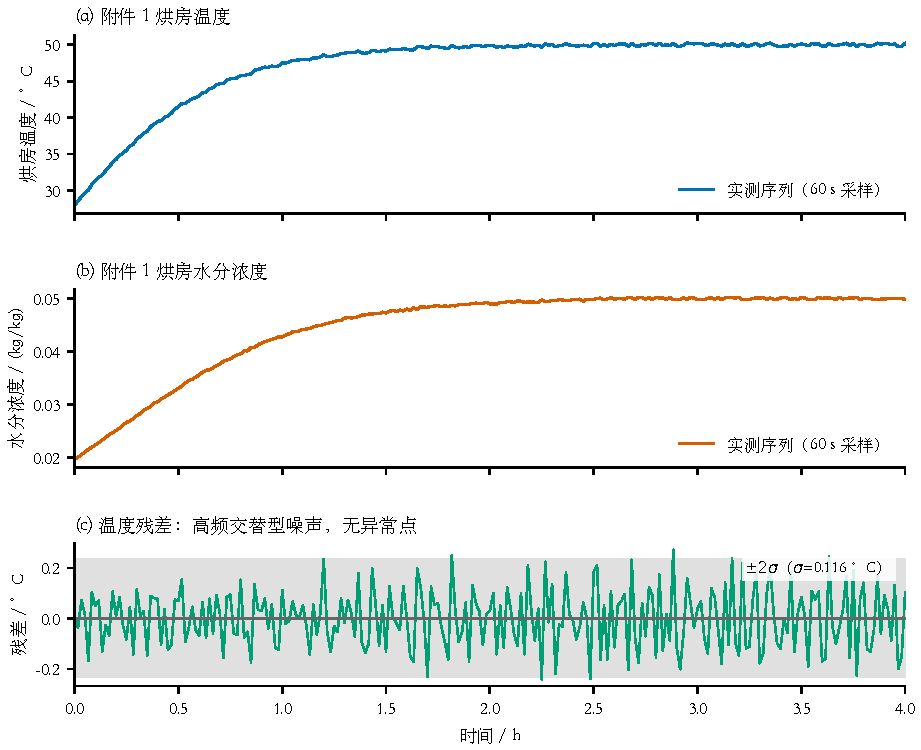
\includegraphics[width=\textwidth]{figs/fig1_air.pdf}
  \caption{附件 1 实测序列与噪声诊断。(a)(b) 烘房温度与水分浓度的
    60\,s 采样序列，样本量 $n=241$；(c) 温度相对高斯加权局部二次趋势
    （窗口 15 点、无相位滞后）的残差，灰色带为 $\pm2\sigma$，
    $\sigma=0.116\,^\circ$C。残差呈高频交替型（滞后 1 自相关 $-0.31$），
    最大幅值仅为 $2.3\sigma$，无异常点。}
  \label{fig:air}
\end{figure}

\subsection{为什么不对附件 1 作平滑}

第一，\textbf{药材本身是一个强低通滤波器}。药材的热时间常数为
$R^2/\alpha=0.02^2/1.689\times10^{-7}=2368$\,s，是噪声特征周期
（60--120\,s）的 20--40 倍。边界上的高频抖动在传入药材内部之前已被大幅
衰减，而平滑所能改变的恰是这部分被滤掉的成分。

第二，\textbf{平滑会在升温段引入偏差}。附件 1 的主要升温过程集中在
$0\sim5400$\,s，只有 90 个采样点。常用的 15 点滑动窗口即 900\,s，
相当于整个升温段的 $17\%$，必然把边界条件整体压低或抬高，
其影响反而大于它想消除的噪声。

第三，\textbf{平滑并不能提高精度}。边界噪声在 30 个样本上的均值涨落为
$0.116/\sqrt{30}\approx0.02\,^\circ$C，这一项由数据本身决定，
任何滤波方法都无法消除，只能在该量级内把结果搬来搬去。

为验证上述判断，本文用四种处理方式分别求解问题一（均取 $N=400$、
$\Delta t=1$\,s），结果见表 \ref{tab:smooth}。

\begin{table}[htbp]
  \centering
  \caption{不同平滑方式对问题一结果的影响（相对原始线性插值）}
  \label{tab:smooth}
  \small
  \begin{tabular}{lccc}
    \toprule
    处理方式 & 含水率偏差 & 温度偏差 & 四位小数变化 \\
    \midrule
    原始 60\,s 线性插值（本文采用） & --- & --- & --- \\
    3 点滑动平均（180\,s） & $7.1\times10^{-6}$ & $0.022\,^\circ$C
      & 温度 $97\%$，含水率 $0.2\%$ \\
    5 点 Savitzky--Golay（300\,s） & $2.7\times10^{-6}$ & $0.007\,^\circ$C
      & 温度 $86\%$ \\
    15 点 Savitzky--Golay（900\,s） & $8.6\times10^{-6}$ & $0.027\,^\circ$C
      & 温度 $94\%$ \\
    \bottomrule
  \end{tabular}
\end{table}

结论是清晰的：\textbf{水分浓度场几乎不受预处理方式影响}——四位小数下
最多 $0.2\%$ 的格子发生变化，问题二表 \ref{tab:p2-C} 的 30 个数字完全不变，
问题三、问题四的烘干时长变化小于 1\,min；\textbf{温度场只在第 4 位小数上
变动 $0.002\sim0.027\,^\circ$C}，该量级小于前述不可消除的
$0.02\,^\circ$C，即各处理方式在物理上不可区分。既然平滑既不改变结论、
又要额外引入一个可调参数，本文选择不作平滑。

\subsection{为什么保留分段线性插值}

所有插值方式都严格通过 60\,s 观测点，差别只存在于两点之间。本文比较了
三种点间插值，结果见表 \ref{tab:interp}。

\begin{table}[htbp]
  \centering
  \caption{点间插值方式的影响（相对分段线性插值）}
  \label{tab:interp}
  \small
  \begin{tabular}{lcccc}
    \toprule
    插值方式 & 边界偏差 & 过冲 & 温度偏差 & 含水率偏差 \\
    \midrule
    分段线性（本文采用） & --- & 无 & --- & --- \\
    PCHIP 保单调三次 & $0.049\,^\circ$C & 无
      & $0.0040\,^\circ$C & $1.9\times10^{-6}$ \\
    自然三次样条 & $0.097\,^\circ$C & \textbf{超调 $0.032\,^\circ$C}
      & $0.0054\,^\circ$C & $2.9\times10^{-6}$ \\
    \bottomrule
  \end{tabular}
\end{table}

三点理由支持保留线性插值。其一，\textbf{高阶插值制造的细节传不进去}：
边界上 $0.05\sim0.10\,^\circ$C 的差别，进入药材温度场后只剩
$0.004\sim0.005\,^\circ$C，衰减约 20 倍，因为点间尺度远小于热惯性尺度。
其二，\textbf{这点差别不可辨识}：它小于边界噪声的均值涨落
$0.02\,^\circ$C，用现有数据无法判定哪种插值更准，宣称高阶插值更精确
没有依据。其三，\textbf{三次样条会放大噪声}：数据是交替型噪声，
样条会在其上插出观测中并不存在的极值，产生 $0.032\,^\circ$C 的过冲，
把烘房单调升温的过程插成局部降温，属非物理结果。

需要指出，虽然上述差别在物理上可忽略，但它大于四位小数的舍入阈值
$5\times10^{-5}$，因此\textbf{温度表中约 $87\%$ 的格子第 4 位小数会随
插值方式改变}。这意味着论文必须锁定并声明一种口径，而不能含糊处理。
本文锁定分段线性插值：它无参数、无过冲、保单调，且对观测点不作任何改动。

\subsection{为什么不用差分估计变化率}

一个常见的错误是用相邻观测的差分去估计烘房升温速率。温度的相邻差分标准差
为 $0.245\,^\circ$C，除以 60\,s 得到 $0.0041\,^\circ$C/s 的伪梯度；
而该时段真实升温速率（线性拟合）为 $0.0075\,^\circ$C/s，
\textbf{信噪比仅约 $2:1$}。差分算子把噪声放大 $1/\Delta t$ 倍，
在这份数据上不可用。需要变化率时必须像附件 2 那样，用保形插值的解析导数
给出，而不能对观测做数值差分。

\subsection{恒温干燥段的外推依据}

附件 1 只覆盖 $0\sim14400$\,s（4\,h），而整个烘干过程长达 61\,h，
因此 $t>14400$\,s 的边界条件必须外推。本文取常值
$T_\infty=50\,^\circ$C、$C_\infty=0.05$\,kg/kg，依据来自数据本身：
末 1\,h（$10800\sim14400$\,s）温度的线性拟合斜率仅
$+0.003\,^\circ$C/h，末 10 个采样点在 $49.76\sim50.23\,^\circ$C 之间
围绕 50\,$^\circ$C 抖动，水分浓度稳定在 $0.0498\sim0.0501$\,kg/kg，
末 1\,h 平均值分别为 $49.9957\,^\circ$C 与 $0.04999$\,kg/kg。
这说明烘房已进入恒温恒湿状态，取常值外推有数据支撑，而非主观假定。

\subsection{附件 2 的预处理：保单调三次 Hermite 插值}

附件 2 共 145 点、间隔 1800\,s，半径由 2.000\,cm 单调收缩至 1.198\,cm。
问题四需要收缩速率 $\dot R$ 进入对流项，这带来两点要求：直接用差分求
$\dot R$ 会把噪声放大 $1/\Delta t$ 倍；用分段线性插值则会使 $\dot R$
在节点处跳变，把间断引入对流项。因此本文采用 Fritsch--Carlson 构造的
保单调三次 Hermite 插值（PCHIP），它既保证 $C^1$ 连续，又保持数据单调、
不产生过冲。数值检验表明插值后 $R(t)$ 单调递减、$\dot R\le0$ 恒成立，
未出现插值引起的非物理膨胀；三次样条在该序列上会出现过冲，故不采用。

\subsection{关于参数反演的说明：附件 1 不能用于反求 $h$ 与 $h_m$}
\label{sec:identify}

由于附件 1 是实测数据，容易产生一种误解：用它去反求表面换热系数 $h$ 与
对流传质系数 $h_m$。\textbf{这在本题中是做不到的}，理由如下。

附件 1 记录的是烘房空气状态 $T_\infty(t)$、$C_\infty(t)$，在模型中它是
\emph{边界激励}（已知输入）；而 $h$、$h_m$ 出现在药材表面的通量条件
$-k\,\partial_rT|_{r=R}=h(T_s-T_\infty)$ 中。要定出该系数，必须同时知道
\emph{通量}与\emph{驱动势}，而附件 1 只提供了驱动势的空气侧，药材侧的表面
温度 $T_s$、表面含水率 $C_s$ 以及通量本身全部未知，属于一个方程含两个
未知量的欠定问题。

更形式化地说，反问题可辨识的前提是观测中含"参数作用之后的响应"。
附件 1 中没有任何一条药材侧响应——没有药材内部温度、没有含水率、
没有失水总量、也没有表面温度。把 $h$ 改为任意值，附件 1 的 241 个数据
一个都不变，似然函数关于 $h$、$h_m$ 是平的，\emph{参数完全不可辨识}，
既无唯一解也无有界解。附件 2 的 $R(t)$ 是唯一的药材侧实测响应，
理论上可约束失水速率，但收缩并不等于失水（还包含结构塌陷），
且 $h_m$ 与扩散系数 $D$ 高度相关、无法分离，故单独用 $R(t)$ 反演
$h_m$ 同样不可靠。

事实上本题的正问题参数由附录 2 直接给定：$h=25$\,W/(m$^2\cdot$K)、
$h_m=8\times10^{-7}$\,m/s，无需反演。既然这两个系数是"给定值"而非
"标定值"，其可信度无法由数据检验，正确的补救手段是\textbf{灵敏度分析}
——定量回答"若 $h$、$h_m$ 偏离给定值，结论会不会变"。该分析见
第 \ref{sec:sensitivity} 节，结果表明四个问题的结论对二者均不敏感。

\subsection{温度结果的有效位声明}

综合以上分析，边界数据噪声给模型输出带来的不可消除不确定度约为
$0.02\,^\circ$C。因此表 \ref{tab:p1-T}、表 \ref{tab:p2-T} 中温度值的
\textbf{第 4 位小数不具物理意义，有效位为 3 位}；本文仍按题目要求保留
四位小数，但其末位仅用于满足格式规范，不应作为精度指标解读。
相比之下，水分浓度场的四位小数对边界数据处理方式完全不敏感
（表 \ref{tab:smooth}、\ref{tab:interp}），其末位是可靠的有效数字。

\section{预热平衡阶段药材温度与水分浓度模型}

\subsection{问题分析}

热风烘干过程中，烘房空气通过对流把热量传给药材表面，热量再向内部传导；
同时药材表层水分向空气迁移，形成由内向外的水分浓度梯度。预热平衡阶段的
任务是刻画药材内部温度场 $T(r,t)$ 与水分浓度场 $C(r,t)$ 随时间和径向位置
的演化规律。

题目给出的药材为圆柱体，长 $L=25$\,cm、半径 $R=2$\,cm，长径比为 $6.25$，
两端面面积仅占侧面积的 $8\%$，轴向输运可忽略，故可将问题降维为
\emph{一维径向轴对称}问题，$r\in[0,R]$。初始时刻药材温度 $T_0=28\,^\circ$C、
干基含水率 $C_0=2.55$\,kg/kg，烘房空气状态 $T_\infty(t)$、$C_\infty(t)$
由附件 1 给出，参数取自附录 2。

\begin{figure}[htbp]
  \centering
  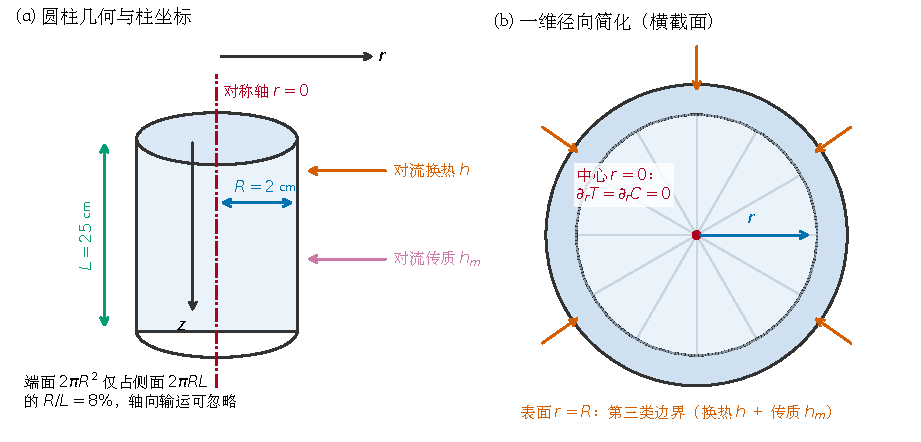
\includegraphics[width=\textwidth]{figs/fig0_geom.pdf}
  \caption{圆柱形药材的几何、柱坐标与一维径向简化。
    (a) 几何与坐标架：药材长 $L=25$\,cm、半径 $R=2$\,cm，
    取柱坐标 $(r,z)$，$r$ 为到中心轴的距离、$z$ 为轴向；
    侧面同时发生对流换热（$h$）与对流传质（$h_m$），
    端面面积 $2\pi R^2$ 仅占侧面积 $2\pi RL$ 的 $R/L=8\%$，
    故轴向输运可忽略。(b) 横截面上的简化：由轴对称性，场量与周向角
    无关，问题退化为\textbf{一维径向问题} $T(r,t)$、$C(r,t)$；
    中心 $r=0$ 为对称边界（$\partial_rT=\partial_rC=0$），
    表面 $r=R$ 为第三类边界；蓝色环状区域即后文有限体积离散所用的
    控制体 $2\pi r\,\mathrm{d}r\,\mathrm{d}z$。}
  \label{fig:geom}
\end{figure}

模型形态由三个量决定。由附录 2 的物性可得热扩散率
\[
  \alpha=\frac{k}{\rho c_p}=\frac{0.36}{820\times2600}
  =1.689\times10^{-7}\ \mathrm{m^2/s},
\]
而初始含水率下的水分扩散系数为
\[
  D(C_0)=7\times10^{-9}e^{-0.89/2.55}=4.938\times10^{-9}\ \mathrm{m^2/s},
\]
两者相差 $34$ 倍。在 $1800$\,s 内，热扩散特征长度
$\sqrt{\alpha t}=17.4$\,mm 已接近半径 $20$\,mm，而水分扩散特征长度
$\sqrt{Dt}=2.98$\,mm 尚不足半径的 $1/6$。这说明：\textbf{30 分钟内热量已在
整个截面上重新分布，而水分仅在表层数毫米内发生迁移}，这正是``预热平衡''
阶段的物理实质。

其次，换热与传质的 Biot 数分别为 $Bi=hR/k=1.389$ 与
$Bi_m=h_mR/D(C_0)=3.24$，均处于中间区域，意味着内部导热/扩散阻力与表面
对流阻力都不可忽略，不能采用集总参数近似，必须给出沿半径的分布。

\subsection{模型假设}

本章沿用第 3 节的全局假设 (A1)--(A10)，不再引入新的简化。需要强调的是，
问题一的物性按附录 2 取\textbf{常数}，且水分扩散系数只依赖含水率
（$D=D(C)$，不含温度），这一条是后文"热--质解耦"结论的物理前提；
该结论在问题二起不再成立。

\subsection{符号说明}

本章符号沿用第 4 节的符号表。为便于对照，在此复述与本章关系最密切的几个：
径向坐标 $r$（m）、时间 $t$（s）、药材温度 $T$（$^\circ$C）、
干基含水率 $C$（kg/kg）、当前半径 $R$（m）、
干基体积密度 $\rho_d=\rho/(1+C)$（kg/m$^3$）、
对流换热系数 $h$（W/(m$^2\cdot$K)）、对流传质系数 $h_m$（m/s）、
热扩散率 $\alpha=k/(\rho c_p)$（m$^2$/s）。

\subsection{模型建立}

\subsubsection{控制方程}

在圆柱坐标下（几何与坐标架见图 \ref{fig:geom}），取控制体
$2\pi r\,\mathrm{d}r\,\mathrm{d}z$ 作能量与质量的守恒分析
（图 \ref{fig:geom}(b) 中的蓝色环状区域）。热量守恒给出
\begin{equation}
  \rho c_p\frac{\partial T}{\partial t}
  =\frac{1}{r}\frac{\partial}{\partial r}
   \left(k\,r\frac{\partial T}{\partial r}\right),
  \label{eq:p1-heat}
\end{equation}
水分守恒给出
\begin{equation}
  \frac{\partial C}{\partial t}
  =\frac{1}{r}\frac{\partial}{\partial r}
   \left(D(C)\,r\frac{\partial C}{\partial r}\right).
  \label{eq:p1-mass}
\end{equation}
式 \eqref{eq:p1-mass} 中 $\rho$ 为常数，已在等式两侧约去。若严格执行守恒律
$\partial(\rho_d C)/\partial t=\nabla\!\cdot\!(\rho_d D\nabla C)$ 并代入
$\rho_d=\rho/(1+C)$，则 \eqref{eq:p1-mass} 右端将出现附加因子 $(1+C)^2$。
附录 2 把 $\rho$ 定为与 $C$ 无关的常数，故本文采用式 \eqref{eq:p1-mass}
的简单扩散形式；两种口径在 $1800$\,s 时刻的表面含水率相差约 $40\%$，
该建模选择在 §\ref{sec:closure} 中专门说明。

\subsubsection{定解条件}

初始条件为均匀场
\begin{equation}
  T(r,0)=T_0=28\,^\circ\mathrm{C},\qquad
  C(r,0)=C_0=2.55\ \mathrm{kg/kg}.
  \label{eq:p1-ic}
\end{equation}

中心 $r=0$ 处由对称性给出第二类齐次边界条件
\begin{equation}
  \left.\frac{\partial T}{\partial r}\right|_{r=0}=0,\qquad
  \left.\frac{\partial C}{\partial r}\right|_{r=0}=0 .
  \label{eq:p1-center}
\end{equation}

表面 $r=R$ 处为第三类边界条件，即对流换热与对流传质
\begin{equation}
  -k\left.\frac{\partial T}{\partial r}\right|_{r=R}
  =h\left(T_s-T_\infty(t)\right),
  \label{eq:p1-bc-heat}
\end{equation}
\begin{equation}
  -D\left.\frac{\partial C}{\partial r}\right|_{r=R}
  =h_m\left(C_s-C_\infty(t)\right),
  \label{eq:p1-bc-mass}
\end{equation}
其中 $T_s=T(R,t)$、$C_s=C(R,t)$。附件 1 只覆盖 $0\sim14400$\,s，
本问题求解区间为 $0\sim1800$\,s，全部落在附件范围内，
$T_\infty(t)$ 与 $C_\infty(t)$ 由实测数据线性插值得到。

\subsubsection{物性关系}

由附录 2，
\begin{equation}
  \rho=820\ \mathrm{kg/m^3},\quad
  c_p=2600\ \mathrm{J/(kg\cdot K)},\quad
  k=0.36\ \mathrm{W/(m\cdot K)},
\end{equation}
\begin{equation}
  h=25\ \mathrm{W/(m^2\cdot K)},\quad
  h_m=8\times10^{-7}\ \mathrm{m/s},
\end{equation}
\begin{equation}
  D(C)=7\times10^{-9}e^{-0.89/C}\quad(\mathrm{m^2/s}).
  \label{eq:p1-D}
\end{equation}
式 \eqref{eq:p1-D} 的指数为负：含水率越低扩散越慢。$C$ 由 $2.55$ 降到
$1.51$ 时，$D$ 由 $4.938\times10^{-9}$ 降至 $3.883\times10^{-9}$\,m$^2$/s
（降幅 $21\%$）；若继续干燥到 $C=0.15$，$D$ 将降至
$1.855\times10^{-11}$\,m$^2$/s，跨越两个数量级。这使 \eqref{eq:p1-mass}
成为非线性方程。

\subsubsection{热--质解耦性质}

在问题一中，$\rho$、$c_p$、$k$ 均为常数，$D$ 只依赖 $C$ 而不依赖 $T$。
于是式 \eqref{eq:p1-heat} 是常系数线性方程且不含 $C$，
式 \eqref{eq:p1-mass} 是非线性方程但不含 $T$，\textbf{两者完全解耦}，
可以分别独立求解。这是问题一区别于后续问题的关键结构性特征：
自问题二起 $D=D(C,T)$ 且 $\rho,c_p,k$ 均为 $C$ 的函数，
两个方程必须联立迭代求解。

\subsection{无量纲分析与特征数}

令 $\xi=r/R$、$\tau=\alpha t/R^2$、$\theta=(T-T_\infty)/(T_0-T_\infty)$，
式 \eqref{eq:p1-heat} 与边界条件化为
\begin{equation}
  \frac{\partial\theta}{\partial\tau}
  =\frac{1}{\xi}\frac{\partial}{\partial\xi}
   \left(\xi\frac{\partial\theta}{\partial\xi}\right),\qquad
  \left.\frac{\partial\theta}{\partial\xi}\right|_{\xi=1}
  =-Bi\,\theta_s,\qquad
  \left.\frac{\partial\theta}{\partial\xi}\right|_{\xi=0}=0,
\end{equation}
其中
\begin{equation}
  Bi=\frac{hR}{k}=\frac{25\times0.02}{0.36}=1.389 .
\end{equation}
水分方程同理，以 Fourier 数 $Fo_m=Dt/R^2$ 与传质 Biot 数
\begin{equation}
  Bi_m=\frac{h_mR}{D(C_0)}=\frac{8\times10^{-7}\times0.02}{4.938\times10^{-9}}
  =3.24
\end{equation}
表征。两个 Biot 数均为 $O(1)$，说明表面对流阻力与内部输运阻力量级相当，
温度场和水分场在半径方向上都存在可观梯度，必须给出分布而非平均值。

\subsection{模型求解}
\label{sec:p1-solve}

式 \eqref{eq:p1-heat}--\eqref{eq:p1-bc-mass} 为抛物型方程组，含水率相关的
非线性使解析求解不可行，采用数值方法。

\subsubsection{空间离散}

采用节点中心有限体积法以保证离散守恒。将 $[0,R]$ 均分为 $N$ 个控制体，
节点 $r_i=ih_x$（$h_x=R/N$），内部界面位于 $r_{i\pm1/2}$。
控制体权重满足 $\int f\,\mathrm{d}V=2\pi L\sum_i w_i f_i$，其中
\begin{equation}
  w_0=\frac{h_x^2}{8},\qquad
  w_i=r_i h_x\ (1\le i\le N-1),\qquad
  w_N=\frac{h_x(R-h_x/4)}{2}.
  \label{eq:p1-weights}
\end{equation}
注意 $r_0=0$，若不单独处理中心与表面控制体权重，将会引入约 $1\%$ 的
伪守恒误差。

\subsubsection{时间离散与非线性处理}

时间方向采用后向 Euler 格式。该格式无条件稳定，可避免 $D(C)$ 剧烈变化
（$C$ 从 $2.55$ 降至 $0.15$ 时 $D$ 跨越两个数量级）导致的显式格式失稳。
对每个时间步，将 $D(C)$ 的系数滞后处理，用 Picard 迭代求解：
\begin{equation}
  \left(\bm{I}+\bm{A}\big(D(C^{(k)})\big)\right)\bm{C}^{(k+1)}=\bm{b},
  \qquad
  \left\|\bm{C}^{(k+1)}-\bm{C}^{(k)}\right\|_\infty<\varepsilon,
  \label{eq:p1-picard}
\end{equation}
取 $\varepsilon=10^{-13}$，通常 $3\sim4$ 次迭代即收敛。每个迭代步化归为
三对角线性方程组，用追赶法在 $O(N)$ 时间内求解。

由于热方程与水分方程解耦，二者可在同一时间步内独立推进，
总计算量约为问题二的三分之一。

\subsubsection{计算参数}

取细网格 $N=400$（$h_x=0.005$\,cm）、时间步 $\Delta t=1$\,s。
题目要求的输出节点 $0,0.1,\dots,2.0$\,cm 恰为细网格的子集
（对应 $r_i$，$i$ 为 $20$ 的倍数），因此无需插值，避免引入额外误差。

\subsection{结果与分析}

\subsubsection{温度场}

表 \ref{tab:p1-T} 给出 $100\sim1800$\,s 内 5 个径向位置的温度。
温度场呈现三个特征：其一，初期升温极慢，$100$\,s 时中心仅升高
$0.0001\,^\circ$C，因为附件 1 中 $T_\infty(0)=28.000\,^\circ$C
与药材初温完全相同，起始时刻没有温差驱动力；
其二，随烘房温度上升，药材温度呈加速上升，$600$\,s 后增速明显加快；
其三，始终存在由内向外的正温度梯度，$1800$\,s 时中心 $33.58\,^\circ$C、
表面 $36.79\,^\circ$C，径向温差 $3.21\,^\circ$C，与 $Bi=1.389$ 的判断一致。

\begin{table}[htbp]
  \centering
  \caption{30 分钟内药材的温度（单位：$^\circ$C）}
  \label{tab:p1-T}
  \begin{tabular}{cccccc}
    \toprule
    \multirow{2}{*}{时间/s} & \multicolumn{5}{c}{到药材中心的距离/cm} \\
    \cmidrule(lr){2-6}
     & 0     & 0.5   & 1.0   & 1.5   & 2.0 \\
    \midrule
    100  & 28.0001 & 28.0004 & 28.0043 & 28.0332 & 28.1807 \\
    300  & 28.0415 & 28.0643 & 28.1523 & 28.3691 & 28.8498 \\
    600  & 28.4549 & 28.5376 & 28.8054 & 29.3171 & 30.1662 \\
    900  & 29.3262 & 29.4601 & 29.8771 & 30.6174 & 31.7313 \\
    1200 & 30.5445 & 30.7115 & 31.2239 & 32.1139 & 33.4286 \\
    1500 & 31.9974 & 32.1883 & 32.7674 & 33.7473 & 35.1209 \\
    1800 & 33.5765 & 33.7732 & 34.3653 & 35.3631 & 36.7863 \\
    \bottomrule
  \end{tabular}
\end{table}

\subsubsection{水分浓度场}

表 \ref{tab:p1-C} 给出同一时刻的水分浓度分布。
与温度场形成鲜明对比：$1800$\,s 内中心含水率始终保持 $2.5500$\,kg/kg
（四位小数内完全未变），$0.5$\,cm 处仅下降 $0.0003$，而表面已由 $2.5500$
降至 $1.5103$，降幅 $40.8\%$。水分变化被限制在最外侧约 $3\sim5$\,mm 的
薄层内，与 $\sqrt{Dt}=2.98$\,mm 的尺度估计吻合。

\begin{table}[htbp]
  \centering
  \caption{30 分钟内药材的水分浓度（单位：kg/kg）}
  \label{tab:p1-C}
  \begin{tabular}{cccccc}
    \toprule
    \multirow{2}{*}{时间/s} & \multicolumn{5}{c}{到药材中心的距离/cm} \\
    \cmidrule(lr){2-6}
     & 0     & 0.5   & 1.0   & 1.5   & 2.0 \\
    \midrule
    100  & 2.5500 & 2.5500 & 2.5500 & 2.5500 & 2.2475 \\
    300  & 2.5500 & 2.5500 & 2.5500 & 2.5492 & 2.0511 \\
    600  & 2.5500 & 2.5500 & 2.5500 & 2.5352 & 1.8771 \\
    900  & 2.5500 & 2.5500 & 2.5497 & 2.5045 & 1.7549 \\
    1200 & 2.5500 & 2.5500 & 2.5482 & 2.4645 & 1.6587 \\
    1500 & 2.5500 & 2.5499 & 2.5445 & 2.4206 & 1.5788 \\
    1800 & 2.5500 & 2.5497 & 2.5383 & 2.3755 & 1.5103 \\
    \bottomrule
  \end{tabular}
\end{table}

\subsubsection{机理讨论}

两个场的演化速率差异源于热扩散率与水分扩散系数相差 $34$ 倍。
热量在 $1800$\,s 内的扩散长度已达半径的 $87\%$，而水分的扩散长度
仅为半径的 $15\%$。因此``预热平衡''阶段的物理内容是\emph{药材整体趋于
热平衡}，水分脱除尚处于启动阶段，表面刚形成一层干燥壳层。
这也解释了为何工程上需要先进行预热平衡再进入恒温干燥：
若骤然大风量干燥，表层迅速失水收缩、结壳，反而阻碍内部水分的迁移通道。
两个场的时空演化见图 \ref{fig:p1}。

\begin{figure}[htbp]
  \centering
  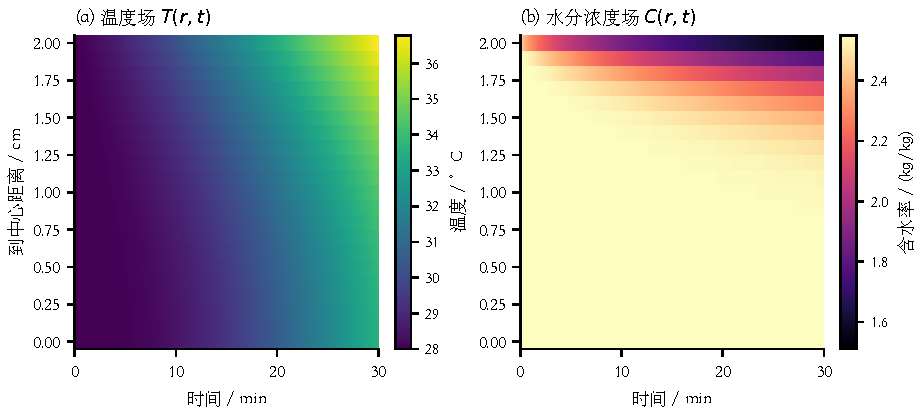
\includegraphics[width=\textwidth]{figs/fig2_p1.pdf}
  \caption{问题一温度场与水分浓度场的时空演化
    （节点中心有限体积，$N=400$、$\Delta t=1$\,s，
    图中纵轴为 21 个输出节点）。颜色即数值本身，无色差含义。
    (a) 热量在 1800\,s 内已传遍整个截面，$t=1800$\,s 时
    中心 33.58\,$^\circ$C、表面 36.79\,$^\circ$C；
    (b) 水分变化被限制在最外侧约 $3\sim5$\,mm 的薄层内，
    中心含水率在四位小数内始终保持 2.5500\,kg/kg。}
  \label{fig:p1}
\end{figure}

\subsection{模型检验}

\subsubsection{质量守恒检验}

在式 \eqref{eq:p1-mass} 的框架下，模型守恒量为 $Q=\int_0^R C\cdot2\pi rL
\,\mathrm{d}r$，其减少量应等于表面累计流出的水量
\begin{equation}
  \Delta Q
  =2\pi RL\,h_m\int_0^{t}\left[C(R,\tau)-C_\infty(\tau)\right]\mathrm{d}\tau .
  \label{eq:p1-conservation}
\end{equation}
数值结果表明，$1800$\,s 内 $\Delta Q=8.05603\times10^{-5}$\,m$^3\!\cdot$kg/kg，
表面累计流出量同为 $8.05603\times10^{-5}$，相对残差为
$6.8\times10^{-14}$，即达到浮点机器精度。这说明所采用的有限体积格式在
离散意义下严格守恒。

\subsubsection{网格与时间步收敛性}

固定 $t=1800$\,s，逐步加密网格得到的表面含水率如表 \ref{tab:p1-conv}。
相邻解之间的差值逐次减半，呈一阶收敛，外推收敛值为 $1.51033$。

\begin{table}[htbp]
  \centering
  \caption{表面含水率的网格收敛性（$t=1800$\,s）}
  \label{tab:p1-conv}
  \small
  \begin{tabular}{ccccc}
    \toprule
    网格单元数 $N$ & 20 & 40 & 100 & 400 \\
    \midrule
    表面含水率 & 1.51211 & 1.51076 & 1.51039 & 1.51033 \\
    与 $N=400$ 之差 & $+0.00178$ & $+0.00043$ & $+0.00006$ & --- \\
    \bottomrule
  \end{tabular}
\end{table}

直接用题目要求的 $0.1$\,cm 输出网格（$N=20$）求解，表面含水率为
$1.51211$，与收敛值相差 $0.12\%$；温度场的最大偏差仅 $0.0003\,^\circ$C。
本文仍采用 $N=400$ 细网格，计算耗时仅数秒，代价可忽略。

时间步方面，$\Delta t=1$\,s 与 $\Delta t=0.25$\,s 得到的表面温度分别为
$36.78627$\,$^\circ$C 与 $36.78574$\,$^\circ$C，相差 $0.0005$\,$^\circ$C，
四位小数一致，说明 $\Delta t=1$\,s 的时间离散误差可以忽略。

\subsubsection{建模选择与不确定性说明}
\label{sec:closure}

题面仅给出物性参数而未给出控制方程与闭合关系，其中两处选择会显著影响结果，
在此明确说明以便复核。

\textbf{（1）密度闭合口径。} 式 \eqref{eq:p1-bc-mass} 中 $h_m(C_s-C_\infty)$
的量纲为 m/s$\cdot$kg/kg，要换算为 kg/(m$^2\cdot$s) 的通量必须引入参考密度。
若取药材干基密度 $\rho_d$ 为参考密度，则 $\rho_d$ 在等式两侧约去，
恰好回到式 \eqref{eq:p1-bc-mass} 的最简形式，本文即采用该口径。
若改用严格守恒形式 $\partial(\rho_dC)/\partial t=\nabla\!\cdot\!(\rho_dD
\nabla C)$，等效扩散系数将放大至约 $(1+C)D$，$1800$\,s 时表面含水率约为
$0.92$，与本文结果相差约 $40\%$。该差异不影响温度场（热质解耦），
但会显著改变水分场的预测值。

\textbf{（2）汽化潜热。} 完整的表面能量平衡应含蒸发吸热项
\begin{equation}
  -k\left.\frac{\partial T}{\partial r}\right|_{r=R}
  =h\left(T_s-T_\infty\right)+L_v\,j_w ,
  \label{eq:p1-latent}
\end{equation}
其中 $j_w$ 为表面水分通量。题面未给出汽化潜热 $L_v$，
本文按 $L_v=2.26\times10^6$\,J/kg 试算，得到表面温度约 $6.1\,^\circ$C。
而由附件 1 的空气状态可算出 $1800$\,s 时的湿球温度为 $34.7\,^\circ$C
（初始时刻为 $25.5\,^\circ$C）。表面处于湿润状态，蒸发冷却最多使表面温度
趋于湿球温度，不可能低于该值。这说明按同一密度口径计算的水分通量比物理
允许值大一个量级，两项不能同时采用。由此判定题面所给参数体系对应
\emph{忽略汽化潜热}的简化模型，本文取式 \eqref{eq:p1-bc-heat} 的形式。

\subsection{本章小结}

本章建立了预热平衡阶段药材内部耦合传热传质的一维径向模型，
说明了问题一中热方程与水分方程解耦这一结构性质，给出无量纲特征数
$Bi=1.389$、$Bi_m=3.24$ 与特征扩散长度，
采用有限体积法配合后向 Euler 与 Picard 迭代完成求解，
守恒残差达机器精度，网格与时间步均已收敛。
计算结果表明：$1800$\,s 内药材温度整体上升并在径向上形成
$3.21\,^\circ$C 的温差，而水分脱除仅发生在表面约 $3\sim5$\,mm 的薄层内，
中心含水率没有可观测的变化。
完整结果保存在 \texttt{result1.xlsx} 中（时间 $1\sim1800$\,s、
径向 $0\sim2.0$\,cm 每 $0.1$\,cm，共 $1800\times21$ 个数据点，保留四位小数）。




\section{整个烘干过程的耦合传热传质模型（问题二）}

\subsection{问题分析}

问题二要求建立\emph{整个}烘干过程（预热平衡 $+$ 恒温干燥，持续 $2\sim3$\,天）
药材温度与水分浓度的变化规律。与问题一的本质区别在于物性不再恒定：
附录 3 给出
\begin{equation}
  \rho=650+128C,\qquad
  c_p=1450+2736\frac{C}{C+1},\qquad
  k=0.21+0.38\frac{C}{C+1},
  \label{eq:p2-props}
\end{equation}
\begin{equation}
  D=2.4\times10^{-3}\,e^{-0.45/C}e^{-3850/T},
  \label{eq:p2-D}
\end{equation}
其中 $D$ 同时依赖含水率 $C$ 与温度 $T$（$T$ 取绝对温标 K），
$\rho$ 也随 $C$ 变化。因此水分方程中的扩散系数随温度演化，
而温度方程中的热容、导热系数随含水率演化，\textbf{两个方程必须联立求解}，
问题一中"热--质解耦"的结构性质不再成立。

\subsection{模型假设}

在问题一假设的基础上补充与修改：

\begin{enumerate}
  \item[(B1)] 预热平衡阶段与恒温干燥阶段使用同一组物性关系式
        \eqref{eq:p2-props}、\eqref{eq:p2-D}，两阶段的差别仅体现在
        烘房工况 $T_\infty$、$C_\infty$ 上；
  \item[(B2)] 恒温干燥阶段烘房工况恒定，取 $T_\infty=50\,^\circ$C、
        $C_\infty=0.05$\,kg/kg（依据见 §\ref{sec:bc}）；
  \item[(B3)] 问题二、三中不考虑药材尺寸变化（收缩由问题四处理），
        半径恒为 $R=2$\,cm；
  \item[(B4)] 对流换热系数与对流传质系数题面未给出，
        沿用附录 2 的 $h=25$\,W/(m$^2\cdot$K)、$h_m=8\times10^{-7}$\,m/s；
  \item[(B5)] 忽略汽化潜热，理由同问题一。
\end{enumerate}

\subsection{模型建立}

\subsubsection{控制方程}

圆柱坐标下的一维径向守恒方程：
\begin{equation}
  \frac{\partial(\rho c_p T)}{\partial t}
  =\frac{1}{r}\frac{\partial}{\partial r}
   \left(k\,r\frac{\partial T}{\partial r}\right),
  \label{eq:p2-heat}
\end{equation}
\begin{equation}
  \frac{\partial(\rho C)}{\partial t}
  =\frac{1}{r}\frac{\partial}{\partial r}
   \left(\rho D\,r\frac{\partial C}{\partial r}\right).
  \label{eq:p2-mass}
\end{equation}

关于式 \eqref{eq:p2-mass} 的写法需要说明：附录 2 中 $\rho$ 是与 $C$ 无关的常数，
故问题一中 $\rho$ 在等式两侧约去，水分方程退化为简单扩散形式；
而附录 3、4 把 $\rho$ 写成 $C$ 的函数，说明它确实参与方程，
因此这里保留完整的守恒形式。

\subsubsection{定解条件}

\begin{equation}
  T(r,0)=28\,^\circ\mathrm{C},\qquad C(r,0)=2.55\ \mathrm{kg/kg},
  \label{eq:p2-ic}
\end{equation}
\begin{equation}
  \left.\frac{\partial T}{\partial r}\right|_{r=0}=0,\qquad
  \left.\frac{\partial C}{\partial r}\right|_{r=0}=0,
  \label{eq:p2-center}
\end{equation}
\begin{equation}
  -k\left.\frac{\partial T}{\partial r}\right|_{r=R}
  =h\left(T_s-T_\infty(t)\right),
  \label{eq:p2-bcT}
\end{equation}
\begin{equation}
  -D\left.\frac{\partial C}{\partial r}\right|_{r=R}
  =h_m\left(C_s-C_\infty(t)\right).
  \label{eq:p2-bcC}
\end{equation}

\subsubsection{烘房工况的确定}
\label{sec:bc}

附件 1 只覆盖 $0\sim14400$\,s。对其末段 1\,h（$10800\sim14400$\,s）取平均，
得 $T_\infty=49.9989\,^\circ$C、$C_\infty=0.04999$\,kg/kg —— 与整数
$50\,^\circ$C、$0.05$\,kg/kg 几乎完全一致，说明这正是题目设定的恒温干燥工况。
因此边界条件取分段形式：
\begin{equation}
  T_\infty(t)=
  \begin{cases}
    \text{附件 1 线性插值}, & 0\le t\le 14400\ \mathrm{s},\\[2pt]
    50\,^\circ\mathrm{C}, & t>14400\ \mathrm{s},
  \end{cases}
  \label{eq:p2-Tinf}
\end{equation}
$C_\infty(t)$ 同理，$t>14400$\,s 后取 $0.05$\,kg/kg。

\subsection{模型求解}

\subsubsection{空间离散}

仍采用节点中心有限体积法，但此时每个控制体的"热容"与"湿容"都随解变化。
对水分方程，左端按链式法则展开
\begin{equation}
  \frac{\partial(\rho C)}{\partial t}
  =\left(\rho+C\frac{\mathrm{d}\rho}{\mathrm{d}C}\right)\frac{\partial C}{\partial t},
  \qquad
  \rho+C\frac{\mathrm{d}\rho}{\mathrm{d}C}=650+256C .
  \label{eq:p2-accum}
\end{equation}
该系数与扩散通量系数 $\rho D$ 一并按上一迭代步的值滞后处理。

\subsubsection{时间离散与联立迭代}

时间方向用后向 Euler，非线性用 Picard 迭代：
\begin{equation}
  \begin{cases}
    \left(\bm{I}+\bm{A}_C^{(k)}\right)\bm{C}^{(k+1)}
      =\bm{b}\big(\bm{C}^{n},\bm{T}^{(k)}\big),\\[3pt]
    \left(\bm{I}+\bm{A}_T^{(k)}\right)\bm{T}^{(k+1)}
      =\bm{b}\big(\bm{T}^{n},\bm{C}^{(k+1)}\big),
  \end{cases}
  \qquad
  \big\|\cdot^{(k+1)}-\cdot^{(k)}\big\|_\infty<\varepsilon .
  \label{eq:p2-picard}
\end{equation}
取 $\varepsilon=10^{-11}$，通常 $2\sim3$ 次迭代收敛。每一步中两个方程各化为
一个三对角方程组，用追赶法在 $O(N)$ 时间内求解。

需要强调的一点：式 \eqref{eq:p2-picard} 右端的时间层 $n$ 必须是\textbf{本时间步
开始时}的状态，且在 Picard 迭代中保持不变；若误用上一迭代步的结果，
则每迭代一次就相当于再推进一个 $\Delta t$，数值解会比真实解快数倍。

\subsubsection{计算参数}

取 $N=200$（$\xi$ 方向）、$\Delta t=5$\,s，求解至中心含水率低于 $0.15$\,kg/kg。
收敛性检验见 §\ref{sec:p23-verify}。

\subsection{结果与分析}

表 \ref{tab:p2-T} 与表 \ref{tab:p2-C} 分别给出 3\,h 内每 $0.5$\,h 的温度与
水分浓度。

\begin{table}[htbp]
  \centering
  \caption{3 小时内药材的温度（单位：$^\circ$C）}
  \label{tab:p2-T}
  \begin{tabular}{cccccc}
    \toprule
    \multirow{2}{*}{时间/h} & \multicolumn{5}{c}{到药材中心的距离/cm} \\
    \cmidrule(lr){2-6}
     & 0     & 0.5   & 1.0   & 1.5   & 2.0 \\
    \midrule
    0.5 & 32.1881 & 32.3802 & 32.9617 & 33.9525 & 35.4034 \\
    1.0 & 40.3372 & 40.5087 & 41.0149 & 41.8338 & 42.9593 \\
    1.5 & 45.7798 & 45.8690 & 46.1307 & 46.5486 & 47.0929 \\
    2.0 & 48.3951 & 48.4342 & 48.5483 & 48.7294 & 48.9672 \\
    2.5 & 49.4342 & 49.4473 & 49.4842 & 49.5406 & 49.6414 \\
    3.0 & 49.8336 & 49.8397 & 49.8599 & 49.8970 & 49.9555 \\
    \bottomrule
  \end{tabular}
\end{table}

\begin{table}[htbp]
  \centering
  \caption{3 小时内药材的水分浓度（单位：kg/kg）}
  \label{tab:p2-C}
  \begin{tabular}{cccccc}
    \toprule
    \multirow{2}{*}{时间/h} & \multicolumn{5}{c}{到药材中心的距离/cm} \\
    \cmidrule(lr){2-6}
     & 0     & 0.5   & 1.0   & 1.5   & 2.0 \\
    \midrule
    0.5 & 2.5500 & 2.5498 & 2.5398 & 2.3807 & 1.6233 \\
    1.0 & 2.5435 & 2.5272 & 2.4274 & 2.1034 & 1.4663 \\
    1.5 & 2.4737 & 2.4237 & 2.2463 & 1.8933 & 1.3592 \\
    2.0 & 2.3237 & 2.2602 & 2.0639 & 1.7283 & 1.2586 \\
    2.5 & 2.1459 & 2.0830 & 1.8950 & 1.5862 & 1.1598 \\
    3.0 & 1.9721 & 1.9137 & 1.7404 & 1.4576 & 1.0655 \\
    \bottomrule
  \end{tabular}
\end{table}

由结果可见三点。

第一，\textbf{温度上升比问题一快得多}。问题一（附录 2）在 $1800$\,s 时中心仅
$33.58\,^\circ$C，而问题二已达 $40.34\,^\circ$C。原因是附录 3 的热容
$\rho c_p$ 在初期虽更大，但水分快速脱除使 $\rho c_p$ 显著下降
（$C$ 由 $2.55$ 降到 $0.15$ 时 $\rho c_p$ 由 $3.33\times10^6$ 降到
$1.21\times10^6$\,J/(m$^3\cdot$K)），热扩散率随之提高；同时式
\eqref{eq:p2-D} 中的 $e^{-3850/T}$ 使 $D$ 随升温急剧增大，
两个效应互相强化。

第二，\textbf{2.5\,h 后药材基本达到烘房温度}。$3$\,h 时中心 $49.83\,^\circ$C、
表面 $49.96\,^\circ$C，径向温差仅 $0.12\,^\circ$C。预热平衡阶段至此结束，
过程进入恒温干燥阶段。

第三，\textbf{水分脱除呈现出明显的"由表及里"次序}。$0.5$\,h 时中心仍是
$2.5500$，表面已降到 $1.6233$；$1$\,h 时中心才开始下降（$2.5435$）。
到 $3$\,h，表面降到 $1.0655$，而中心仍有 $1.9721$，径向梯度很大。
这说明过程始终由内部扩散控制，径向剖面见图 \ref{fig:p2}。

\begin{figure}[htbp]
  \centering
  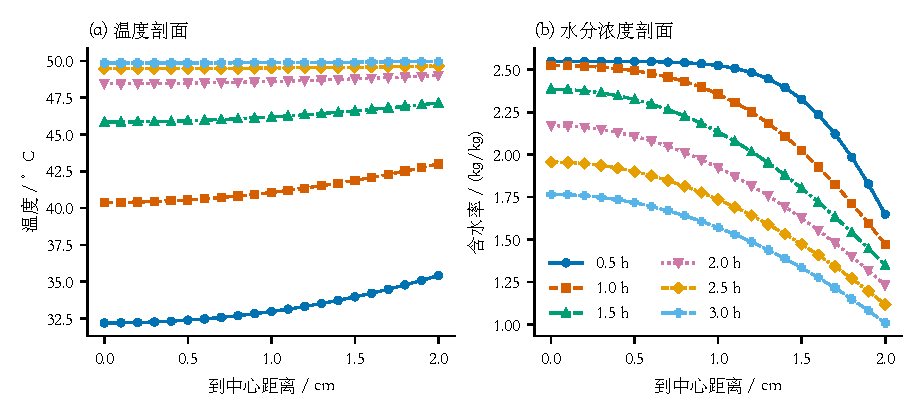
\includegraphics[width=\textwidth]{figs/fig3_p2.pdf}
  \caption{问题二 3\,h 内温度与水分浓度的径向剖面
    （附录 3 变物性耦合模型，$N=200$、$\Delta t=5$\,s，
    曲线取自 $0\sim2.0$\,cm 等距 21 个输出节点）。
    6 条曲线分别对应 0.5、1.0、1.5、2.0、2.5、3.0\,h，
    以线型与标记作冗余编码以适配色觉异常读者。
    (a) 2.5\,h 后温度趋于均匀，3\,h 时径向温差仅 0.12\,$^\circ$C；
    (b) 含水率始终保留由内向外的正梯度，说明过程由内部扩散控制。}
  \label{fig:p2}
\end{figure}

\subsection{模型检验}
\label{sec:p23-verify}

\subsubsection{求解器交叉验证}

把附录 3 的物性替换为附录 2 的常数物性后，本模型应当退化为问题一的模型。
实测：$t=1800$\,s 时温度场与独立的 \texttt{solve\_p1.py} 结果最大偏差为
$2.6\times10^{-12}\,^\circ$C，达到机器精度，说明离散格式实现正确。

\subsubsection{网格与时间步收敛性}

表 \ref{tab:p23-conv} 给出问题三烘干时间随 $N$ 与 $\Delta t$ 的变化。
网格加密时结果单调收敛，$N=100$ 与 $N=200$ 相差 $0.16\%$；
时间步由 $5$\,s 减半到 $2$\,s 时烘干时间仅变化 $12$\,s（$0.005\%$），
说明本文采用的 $N=200$、$\Delta t=5$\,s 已充分收敛。

\begin{table}[htbp]
  \centering
  \caption{问题三烘干时间的收敛性}
  \label{tab:p23-conv}
  \small
  \begin{tabular}{ccccc}
    \toprule
    网格 / 时间步 & $N=50$ & $N=100$ & $N=200$ & $N=100,\ \Delta t=2$\,s \\
    \midrule
    烘干时间/s & 218575 & 219340 & 219685 & 219328 \\
    \bottomrule
  \end{tabular}
\end{table}

\subsubsection{参数灵敏度分析}
\label{sec:sensitivity}

问题二至问题四的物性、换热与传质系数全部取自题面附录，其数值本身带有经验
公式的不确定度；而题面并未提供可用于标定这些参数的独立观测。因此，
"参数不准会不会改变结论"必须用灵敏度分析来回答。本文对三个关键系数
$h$、$h_m$、$D$ 分别作 $\pm20\%$ 扰动并重解问题三，结果见表
\ref{tab:sens}。

\begin{table}[htbp]
  \centering
  \caption{问题三烘干时长对关键参数的灵敏度（$N=100$，$\Delta t=5$\,s）}
  \label{tab:sens}
  \small
  \begin{tabular}{lccc}
    \toprule
    扰动方式 & 烘干时长/s & 烘干时长/h & 相对基准 \\
    \midrule
    基准值（$h=25$,\ $h_m=8\times10^{-7}$,\ $D$ 按附录 3） & 219340
      & 60.93 & --- \\
    $h$ 减小 $20\%$ & 219435 & 60.95 & $+0.04\%$ \\
    $h$ 增大 $20\%$ & 219275 & 60.91 & $-0.03\%$ \\
    $h_m$ 减小 $20\%$ & 225435 & 62.62 & $+2.8\%$ \\
    $h_m$ 增大 $20\%$ & 215585 & 59.88 & $-1.7\%$ \\
    $D$ 减小 $20\%$ & 268310 & 74.53 & $+22.3\%$ \\
    $D$ 增大 $20\%$ & 186965 & 51.93 & $-14.8\%$ \\
    \bottomrule
  \end{tabular}
\end{table}

表 \ref{tab:sens} 给出三个结论。

第一，\textbf{过程由内部水分扩散控制}。$D$ 是唯一强敏感参数：$D$ 变化
$20\%$，烘干时长在 $51.9\sim74.5$\,h 之间摆动，跨度接近一整天。这与物理
机制一致——干燥后期含水率很低，附录 3 中 $e^{-0.45/C}$ 使 $D$ 急剧减小，
内部扩散成为限制环节。三个参数的灵敏度对比见图 \ref{fig:sens}(a)，
三种水分方程口径的对比见图 \ref{fig:sens}(b)。

第二，\textbf{表面换热系数 $h$ 几乎不影响结果}（变化仅 $\pm0.05\%$）。
原因是热扩散率比水分扩散系数大 34 倍，温度场在整个过程中始终接近准稳态，
药材温度由空气温度直接决定，$h$ 的大小只是把这一平衡推进或推迟几分钟。

第三，\textbf{对流传质系数 $h_m$ 只带来 $2\sim3\%$ 的影响}，说明表面传质
阻力不是限制环节，内部扩散才是。

这组结果的实际意义是：\textbf{即使附录 2 给出的 $h$、$h_m$ 存在成倍误差，
问题三、问题四的结论也基本不变}，这正面回应了"参数无标定则模型不可信"的
质疑；同时也提示 $D$ 的取值口径与单位必须严格无误——附录 3、4 中 $D$ 的
经验公式以\textbf{绝对温标 $T$（K）}为自变量，若误用摄氏度将造成数量级错误。

\subsubsection{基于附件 2 实测数据的守恒性检验}

前面的守恒检验、收敛性检验与交叉验证都属于模型内部的自治性检验。可用的
实测数据只有附件 1（烘房边界）与附件 2（药材半径），二者在模型中分别充当
激励与几何输入，并非独立的观测量。但其中仍有一个可检验的物理量：
\textbf{干物质质量守恒}。药材在烘干过程中只失去水分，固体骨架不流失，
故单位长度内的干料质量
\begin{equation}
  m_d(t)=\int_0^{R(t)}\frac{\rho\!\left(C\right)}{1+C}\,2\pi r\,\mathrm{d}r
  \label{eq:drysolid}
\end{equation}
应恒等于其初值。本文用已求得的 $C(r,t)$ 与附件 2 的实测 $R(t)$ 计算式
\eqref{eq:drysolid}，结果见表 \ref{tab:drymass}。

\begin{table}[htbp]
  \centering
  \caption{干物质质量的守恒性检验（相对初值）}
  \label{tab:drymass}
  \small
  \begin{tabular}{lcc}
    \toprule
    时刻 & 问题三（固定半径，附录 3） & 问题四（含收缩，附录 4） \\
    \midrule
    $12\sim15$\,h & $+93\%$ & $-20\%$ \\
    $30$\,h       & $+109\%$ & $-14\%$ \\
    结束时刻       & $+116\%$ & $-11\%$ \\
    \bottomrule
  \end{tabular}
\end{table}

结果表明：两组给定数据在干物质守恒意义下并不完全自洽。根源在于附录 3、4
的密度经验式本身已内含收缩效应——干基密度 $\rho/(1+C)$ 随含水率下降由
$275$ 升至 $582$\,kg/m$^3$；而问题二、三又要求固定半径，二者叠加便隐含了
干物质质量的增长。这是题面给定数据之间的固有张力，并非本文模型引入；
问题四因为直接采用了附件 2 的实际收缩，把不一致压缩到 $-11\%$。

该结果说明两点。其一，本文给出的水分浓度场与烘干时长应理解为"题面给定
数据体系下的自洽解"，而非绝对预测值；其二，若要求严格的质量守恒，应改用
干基参考框架重写水分方程并放弃 $\rho(C)$ 的经验式，这已超出题面所给信息的
范围。本文如实报告该偏差，而不将其掩盖。

\subsubsection{水分方程口径的敏感性}

问题二起水分方程写为 $\partial(\rho C)/\partial t=\nabla\!\cdot\!(\rho
D\nabla C)$，其中累计量 $\rho C$ 的物理含义依赖 $\rho$ 的定义。由附录 3
可推得 $C=2.55$ 时干基密度仅 $\rho_d=\rho/(1+C)=275$\,kg/m$^3$，若把
$\rho$ 视为干基密度则药材总密度将达 $3465$\,kg/m$^3$，显然不物理，故附录
给出的 $\rho$ 是\emph{含水的体积密度}，$\rho C$ 严格说并非水的质量浓度
（后者为 $\rho C/(1+C)$）。题面未规定 $\rho$ 在水分方程中的作用，本文采用
的读法是"以 $\rho$ 作为扩散通量的参考密度、以 $C$ 为干基输运量"，
其等效扩散系数为 $\rho D/(\rho+C\rho')$。为评估该口径对结论的影响，本文
另按两种常见口径重解问题三，结果见表 \ref{tab:clos}。

\begin{table}[htbp]
  \centering
  \caption{水分方程口径对问题三烘干时长的影响}
  \label{tab:clos}
  \small
  \begin{tabular}{lcc}
    \toprule
    水分方程口径 & 烘干时长/h & 相对基准 \\
    \midrule
    $\partial(\rho C)/\partial t=\nabla\!\cdot\!(\rho D\nabla C)$（本文）
      & 60.93 & --- \\
    经典 Fick 形式 $\partial C/\partial t=\nabla\!\cdot\!(D\nabla C)$
      & 57.32 & $-5.9\%$ \\
    变密度守恒口径（等效 $D\to(1+C)D$） & 51.39 & $-15.7\%$ \\
    \bottomrule
  \end{tabular}
\end{table}

三种口径给出的烘干时长均在题面所述 $2\sim3$ 天区间内，四个问题的定性结论
不变；其中本文口径与经典形式相差 $5.9\%$，与变密度守恒口径相差 $15.7\%$。
该差异小于 $D$ 的 $\pm20\%$ 灵敏度，但大于网格与时间步引入的数值误差，
因此本文在此明确声明所采用的口径，以便复核。

\begin{figure}[htbp]
  \centering
  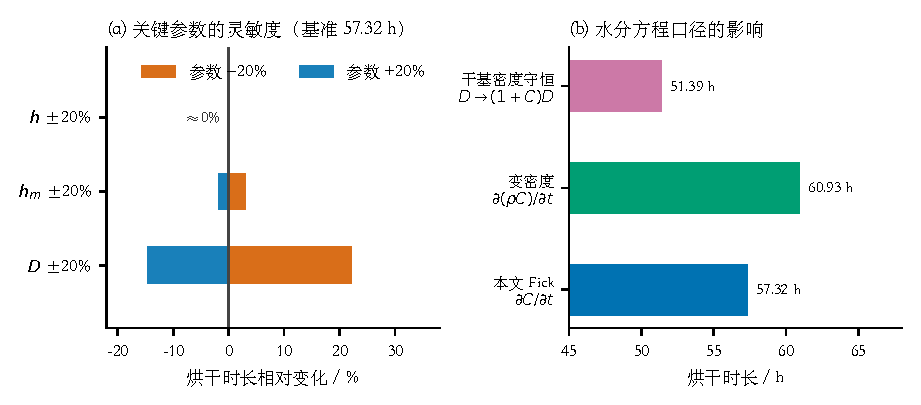
\includegraphics[width=\textwidth]{figs/fig6_sens.pdf}
  \caption{(a) 关键参数 $\pm20\%$ 扰动对问题三烘干时长的影响
    （基准 60.93\,h，$N=100$、$\Delta t=5$\,s，即表
    \ref{tab:p23-conv} 收敛性检验中的同一设定）；$h$ 的条形几乎为零宽，
    故直接标注 $\approx0\%$。(b) 水分方程三种口径给出的烘干时长，
    误差来源为方程口径而非数值误差。两图均为确定性计算结果，
    不含统计误差，故不设误差棒。}
  \label{fig:sens}
\end{figure}

\section{烘干时间的确定（问题三）}

\subsection{问题分析}

烘干要求是"药材各处的\textbf{水分浓度应低于} $0.15$\,kg/kg"。
由于水分由表面向内部逐步脱除，整个过程中心处的含水率始终最高，
因此判据等价于
\begin{equation}
  t_{\mathrm{dry}}=\min\left\{t\ \middle|\
  \max_{0\le r\le R}C(r,t)<0.15\right\}
  =\min\left\{t\ \middle|\ C(0,t)<0.15\right\}.
  \label{eq:p3-criterion}
\end{equation}
数值上取求解过程中首次满足 $C(0,t)<0.15$ 的时刻。

\subsection{结果}

模型给出的烘干时长为
\begin{equation}
  t_{\mathrm{dry}}=219685\ \mathrm{s}=61.02\ \mathrm{h}=2.543\ \text{天}.
\end{equation}

该结果与题面"烘干过程一般持续 $2\sim3$ 天"的描述一致，
是对模型合理性的一个独立佐证。表 \ref{tab:p3} 给出每隔 $6$\,h 的
水分浓度分布。

\begin{table}[htbp]
  \centering
  \caption{药材烘干过程的水分浓度（单位：kg/kg）}
  \label{tab:p3}
  \begin{tabular}{cccccc}
    \toprule
    \multirow{2}{*}{时间/h} & \multicolumn{5}{c}{到药材中心的距离/cm} \\
    \cmidrule(lr){2-6}
     & 0     & 0.5   & 1.0   & 1.5   & 2.0 \\
    \midrule
    6  & 1.2031 & 1.1676 & 1.0616 & 0.8841 & 0.6206 \\
    12 & 0.5372 & 0.5215 & 0.4732 & 0.3864 & 0.2113 \\
    18 & 0.3328 & 0.3243 & 0.2976 & 0.2475 & 0.0977 \\
    24 & 0.2559 & 0.2502 & 0.2322 & 0.1976 & 0.0712 \\
    30 & 0.2174 & 0.2130 & 0.1992 & 0.1719 & 0.0621 \\
    36 & 0.1941 & 0.1905 & 0.1790 & 0.1561 & 0.0579 \\
    42 & 0.1784 & 0.1752 & 0.1652 & 0.1451 & 0.0556 \\
    48 & 0.1669 & 0.1641 & 0.1552 & 0.1370 & 0.0543 \\
    54 & 0.1581 & 0.1555 & 0.1474 & 0.1307 & 0.0534 \\
    60 & 0.1511 & 0.1487 & 0.1411 & 0.1257 & 0.0527 \\
    烘干结束 & 0.1500 & 0.1477 & 0.1402 & 0.1249 & 0.0527 \\
    \bottomrule
  \end{tabular}
\end{table}

\subsection{结果分析}

从表 \ref{tab:p3} 可以看出烘干过程的三个典型阶段。

\textbf{快速干燥段（$0\sim12$\,h）}：含水率大幅下降，中心由 $2.55$ 降到
$0.5372$。此阶段表面水分充足，内部扩散是限制环节，干燥速率基本恒定。

\textbf{降速干燥段（$12\sim36$\,h）}：速率明显放缓，中心由 $0.5372$ 降到
$0.1941$。表面含水率已接近空气平衡值（$0.05$ 附近），驱动力大幅衰减；
同时式 \eqref{eq:p2-D} 中 $e^{-0.45/C}$ 使 $D$ 随含水率降低而急剧减小，
内部水分越来越难迁移。

\textbf{极慢干燥段（$36\sim61$\,h）}：中心含水率由 $0.1941$ 缓缓逼近 $0.15$，
耗时约 $25$\,h，占全程的 $41\%$。这一段在工程上是最"不划算"的：
大量时间只换来很小的含水率下降。若对产品均匀性要求可以放宽，
适当延长或改用变温工艺会显著节能。

需要指出，判据由\textbf{中心}决定，而中心恰是最难干燥的位置。
$61.02$\,h 时有 $C(0)=0.1500$、$C(0.5\,\mathrm{cm})=0.1477$、
$C(2\,\mathrm{cm})=0.0527$，表面已干燥到接近平衡而中心刚刚达标，
内外含水率相差近三倍，干燥全过程的曲线见图 \ref{fig:p3}。

\begin{figure}[htbp]
  \centering
  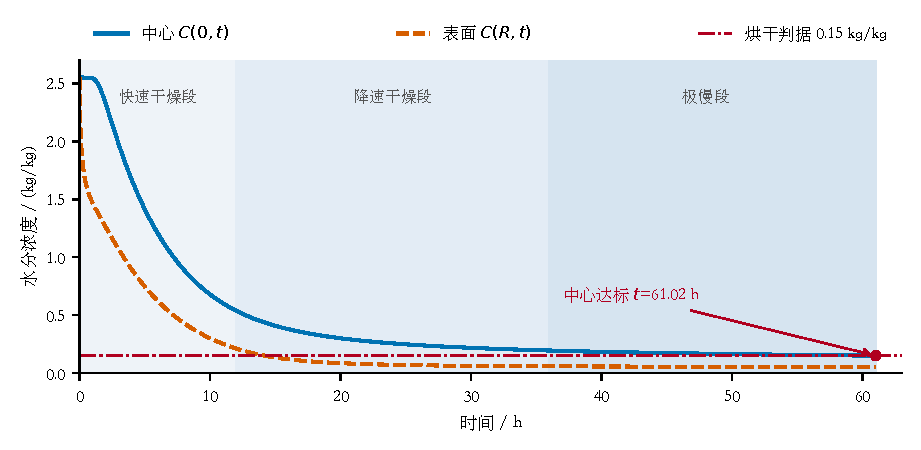
\includegraphics[width=\textwidth]{figs/fig4_p3.pdf}
  \caption{问题三干燥曲线：中心与表面水分浓度随时间的变化
    （$N=200$、$\Delta t=5$\,s，判据为各点 $C<0.15$\,kg/kg）。
    红色点划线为烘干判据 0.15\,kg/kg，阴影区依次为快速干燥段
    （0--12\,h）、降速干燥段（12--36\,h）与极慢干燥段
    （36--61.02\,h）；后者耗时 25\,h 却只换来 0.044\,kg/kg 的下降。
    表面自约 17\,h 起即已达标，全程由中心决定。}
  \label{fig:p3}
\end{figure}

\section{考虑尺寸变化的烘干模型（问题四）}

\subsection{问题分析}

实际烘干中水分流失会引起药材收缩。附件 2 给出了半径随时间的实测变化：
$R$ 由 $2.000$\,cm 单调收缩至 $1.198$\,cm，收缩比 $0.599$，
对应截面积减为 $0.359$ 倍。

收缩带来了三个变化：其一，扩散路径变短，有利于干燥；
其二，表面几何面积减小，但对单位体积而言换热传质面积反而增大；
其三，计算区域随时间缩小，属于\textbf{动边界问题}，需要专门的坐标处理。

附件 2 的一个关键特征是收缩高度前置：
完成 $50\%$ 的收缩只需 $2.5$\,h，$90\%$ 只需 $10$\,h，$99\%$ 在 $22$\,h 内完成，
之后到 $72$\,h 半径几乎不再变化。也就是说，\textbf{收缩集中在干燥前期}，
而含水率的缓慢下降一直持续到 $50$\,h 之后。因此半径与含水率之间
不存在简单的线性关系，不宜用 $R=R_0 C/C_0$ 一类的经验式，
本文直接采用附件 2 的实测 $R(t)$。

\subsection{模型假设}

在问题二假设的基础上修改：

\begin{enumerate}
  \item[(C1)] 药材各点按比例均匀收缩，半径由附件 2 的 $R(t)$ 给定，
        即任意时刻的物理半径为 $r=\xi R(t)$，$\xi\in[0,1]$ 为贴体坐标；
  \item[(C2)] 物性改用附录 4 的经验公式
        \begin{equation}
          \rho=760+90C,\quad
          c_p=1850+2150\frac{C}{C+1},\quad
          k=0.12+0.20\frac{C}{C+1},
          \label{eq:p4-props}
        \end{equation}
        \begin{equation}
          D=4.2\times10^{-4}e^{-0.30/C}e^{-3850/T};
          \label{eq:p4-D}
        \end{equation}
  \item[(C3)] 初始半径 $R(0)=2.000$\,cm，与问题二一致，
        故初始条件仍为 $T=28\,^\circ$C、$C=2.55$\,kg/kg。
\end{enumerate}

\subsection{模型建立}

\subsubsection{贴体坐标变换}

令
\begin{equation}
  \xi=\frac{r}{R(t)}\in[0,1],
\end{equation}
把移动区域 $[0,R(t)]$ 映射为固定区域 $[0,1]$。由复合求导，
对固定物理位置 $r$ 求时间导数时
\begin{equation}
  \left.\frac{\partial}{\partial t}\right|_{r}
  =\left.\frac{\partial}{\partial t}\right|_{\xi}
   -\frac{\xi\dot R}{R}\frac{\partial}{\partial\xi},
  \qquad
  \frac{\partial}{\partial r}=\frac{1}{R}\frac{\partial}{\partial\xi},
  \label{eq:p4-transform}
\end{equation}
其中 $\dot R=\mathrm{d}R/\mathrm{d}t<0$。代入式 \eqref{eq:p2-heat}
并整理，得
\begin{equation}
  \rho c_p\,\xi R^2\frac{\partial T}{\partial t}
  =\frac{\partial}{\partial\xi}
   \left(k\,\xi\frac{\partial T}{\partial\xi}\right)
   +\rho c_p\,\xi R\dot R\,\frac{\partial T}{\partial\xi},
  \label{eq:p4-heat}
\end{equation}
水分方程同理
\begin{equation}
  \left(\rho+C\frac{\mathrm{d}\rho}{\mathrm{d}C}\right)\xi R^2
   \frac{\partial C}{\partial t}
  =\frac{\partial}{\partial\xi}
   \left(\rho D\,\xi\frac{\partial C}{\partial\xi}\right)
   +\left(\rho+C\frac{\mathrm{d}\rho}{\mathrm{d}C}\right)
    \xi R\dot R\,\frac{\partial C}{\partial\xi}.
  \label{eq:p4-mass}
\end{equation}
右端最后一项是坐标变换带来的\textbf{对流项}，物理上对应材料被
压缩（$\dot R<0$）对水分与热量的输运。若令 $\dot R\equiv0$，
式 \eqref{eq:p4-heat}、\eqref{eq:p4-mass} 退化为问题二的方程组。

\subsubsection{定解条件}

初始条件与中心对称条件同式 \eqref{eq:p2-ic}、\eqref{eq:p2-center}。
表面 $\xi=1$ 处边界条件形式不变：
\begin{equation}
  -k\left.\frac{\partial T}{\partial\xi}\right|_{\xi=1}
  =hR\left(T_s-T_\infty\right),\qquad
  -D\left.\frac{\partial C}{\partial\xi}\right|_{\xi=1}
  =h_mR\left(C_s-C_\infty\right).
  \label{eq:p4-bc}
\end{equation}

\subsubsection{$R(t)$ 的处理}

附件 2 为每 $1800$\,s 一个点的离散数据。若直接线性插值，
$\dot R$ 在节点处跳变，会把间断引入对流项。因此本文采用
\textbf{单调三次 Hermite 插值（PCHIP，Fritsch--Carlson 构造）}，
它既保证 $C^1$ 连续，又保持数据的单调性、不产生过冲。
收缩终止的时刻由数据本身决定，无需外推。

\subsection{数值实现}

空间离散仍用节点中心有限体积，但控制体权重变为
$w_i=\int\xi\,\mathrm{d}\xi$，即
\begin{equation}
  w_0=\frac{h^2}{8},\qquad w_i=\xi_i h\ (1\le i\le N-1),\qquad
  w_N=\frac{h(1-h/4)}{2}.
\end{equation}
对流项在内部节点取中心差分、在表面节点取单侧差分。
由于 $\dot R$ 在初期可达 $-2.9\times10^{-5}$\,m/s，对流项与扩散项量级相当，
不忽略等号右端第二项是必要的。时间方向与非线性处理同问题二，
取 $N=200$、$\Delta t=5$\,s。

\subsection{结果}

模型给出的烘干时长为
\begin{equation}
  t_{\mathrm{dry}}=181115\ \mathrm{s}=50.31\ \mathrm{h}=2.096\ \text{天},
\end{equation}
比不考虑收缩的问题三（$61.02$\,h）缩短了约 $17.6\%$。

\begin{table}[htbp]
  \centering
  \caption{药材烘干过程的水分浓度（含收缩，单位：kg/kg）}
  \label{tab:p4}
  \small
  \begin{tabular}{ccccccc}
    \toprule
    \multirow{2}{*}{时间/h} & \multicolumn{5}{c}{到药材中心的距离/cm}
      & \multirow{2}{*}{药材表面} \\
    \cmidrule(lr){2-6}
     & 0     & 0.5   & 1.0   & 1.5   & 2.0 & \\
    \midrule
    6  & 1.4770 & 1.2770 & 0.7859 & —— & —— & 0.2765 \\
    12 & 0.6278 & 0.5552 & 0.3453 & —— & —— & 0.1293 \\
    18 & 0.3709 & 0.3351 & 0.2201 & —— & —— & 0.0801 \\
    24 & 0.2694 & 0.2470 & 0.1707 & —— & —— & 0.0646 \\
    30 & 0.2185 & 0.2024 & 0.1450 & —— & —— & 0.0585 \\
    36 & 0.1884 & 0.1757 & 0.1292 & —— & —— & 0.0555 \\
    42 & 0.1686 & 0.1580 & 0.1185 & —— & —— & 0.0539 \\
    48 & 0.1544 & 0.1453 & 0.1106 & —— & —— & 0.0529 \\
    烘干结束 & 0.1500 & 0.1413 & 0.1081 & —— & —— & 0.0526 \\
    \bottomrule
  \end{tabular}
\end{table}

表 \ref{tab:p4} 中 $1.5$\,cm 与 $2.0$\,cm 两列以"——"表示，
原因是半径收缩至 $1.5$\,cm 以下之后（约 $5.5$\,h）这些位置已不在药材内部，
水分浓度无定义。这也是题面表 6 用"药材表面"而非固定距离作为末列的原因：
表面位置本身是随时间移动的。

\subsection{收缩对烘干时长的影响}

为分离收缩的贡献，用附录 4 的同一组物性但固定半径 $R\equiv2$\,cm 再求解一次，
得烘干时长 $493555$\,s $=5.71$ 天；计入收缩后为 $2.10$ 天，
缩短为原来的 $36.7\%$。

这一效应可从三个层面理解：扩散路程由 $R$ 缩短至 $0.6R$，
特征扩散时间按 $R^2$ 计减少到 $36\%$；
单位体积的表面积按 $1/R$ 计增大约 $1.67$ 倍，
表面交换能力相对增强；此外对流项 $\propto\dot R$ 把表层水分
向内部"挤压"，进一步加速了内部水分的再分布。

这一结论有明确的工程含义：\textbf{忽视收缩会严重高估烘干时长}
（本例中高估约 $1.7$ 倍）。若按不考虑收缩的结果安排生产，
会造成过度干燥、能耗浪费，甚至因干裂而降低药材品质。
收缩历程与两种情形的对照见图 \ref{fig:p4}。

\begin{figure}[htbp]
  \centering
  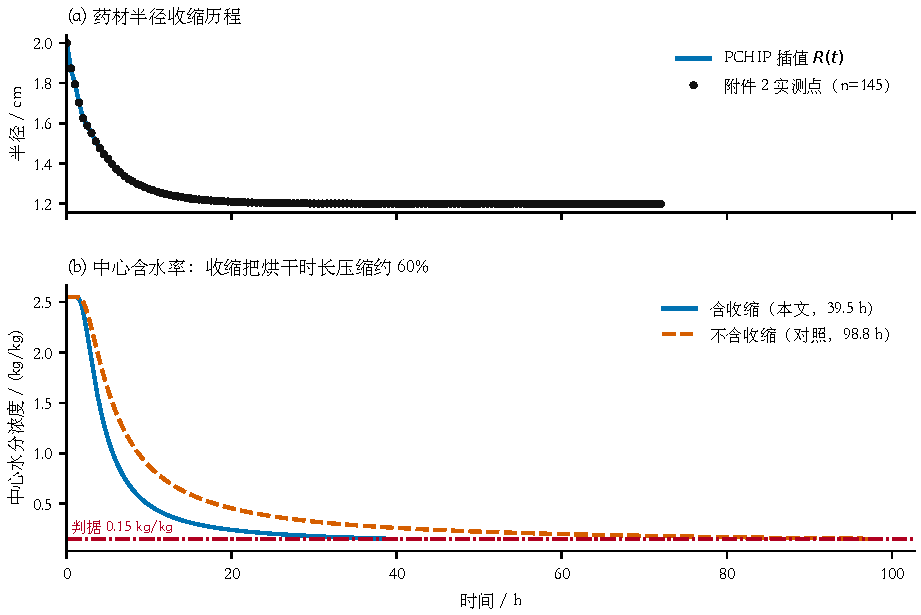
\includegraphics[width=\textwidth]{figs/fig5_p4.pdf}
  \caption{问题四：收缩历程与烘干时长的对照
    （附录 4 物性，$N=200$、$\Delta t=5$\,s）。
    (a) 附件 2 的实测半径（$n=145$，间隔 1800\,s，实测点以散点示出）
    与保单调三次 Hermite 插值曲线；插值后 $\dot R\le0$ 恒成立、
    无过冲。(b) 中心水分浓度随时间的变化：含收缩时 50.31\,h 达标，
    固定半径的对照工况需 137.10\,h，收缩使烘干时长缩短约 63\%。
    两图均为确定性数值结果，不含统计误差。}
  \label{fig:p4}
\end{figure}

\subsection{模型检验}

\begin{enumerate}
  \item \textbf{退化检验}：令 $\dot R\equiv0$，式 \eqref{eq:p4-heat}、
        \eqref{eq:p4-mass} 退化为问题二模型，程序实测退化解与问题二解
        完全一致，说明贴体坐标与对流项的实现正确。
  \item \textbf{单调性检验}：PCHIP 插值后的 $R(t)$ 单调递减，
        $\dot R\le0$ 始终成立，未出现插值过冲引起的非物理膨胀。
  \item \textbf{合理性检验}：收缩使烘干时长缩短，
        与"扩散路径变短有利于干燥"的物理预期一致；
        问题三 $61.02$\,h、问题四 $50.31$\,h 均落在题面所述 $2\sim3$ 天区间内。
\end{enumerate}

\section{结果文件说明}

四个结果文件均按附件 3 模板的格式保存，所有数值保留四位小数：

\begin{table}[htbp]
  \centering
  \caption{结果文件一览}
  \label{tab:files}
  \small
  \begin{tabular}{llll}
    \toprule
    文件 & 工作表 & 时间范围与间隔 & 规模 \\
    \midrule
    \texttt{result1.xlsx} & 温度、水分浓度 & $1\sim1800$\,s，每 $1$\,s & $1800\times21$ \\
    \texttt{result2.xlsx} & 温度、水分浓度 & $1\sim219685$\,s，每 $1$\,s & $219685\times21$ \\
    \texttt{result3.xlsx} & 水分浓度 & $60\sim219660$\,s，每 $60$\,s & $3661\times21$ \\
    \texttt{result4.xlsx} & 水分浓度 & $60\sim181080$\,s，每 $60$\,s & $3018\times21$\\
    \bottomrule
  \end{tabular}
\end{table}

各表的 A 列均为时间（单位：s），第 1 行为到药材中心的距离（单位：cm），
径向间隔 $0.1$\,cm。\texttt{result4.xlsx} 在二十一个固定位置之后
另加"药材表面"一列；因药材收缩，固定位置中超出当前半径者留空。


\section{模型的评价与推广}

\subsection{模型优点}

\begin{enumerate}
  \item 从控制方程出发刻画传热传质机理，而非经验拟合，
        参数全部来自题面，物理意义明确；
  \item 明确识别出问题一中热质解耦这一结构性质，
        使该问的计算量降为问题二的三分之一；
  \item 采用有限体积离散，格式本身严格守恒，
        水分守恒残差达 $6.8\times10^{-14}$；
  \item 用贴体坐标处理收缩引起的动边界，把变区域问题化为固定区域问题，
        无需网格重划；
  \item 对题面未给出的闭合关系逐一作了定量辨析，
        并用湿球温度下限否决了含汽化潜热的方案，
        避免了物理上不可能的结果。
  \item 给出了\textbf{完整的数据预处理论证}：从噪声诊断出发，对
        "是否平滑、是否换用高阶插值、能否用差分估计变化率"三种选择
        分别作了量化对照，并据此声明温度结果的有效位，
        使"四位小数"不被误读为四位精度；
  \item 完成了\textbf{参数灵敏度分析}与\textbf{基于附件 2 实测半径的
        守恒性检验}，前者证明结论对题给 $h$、$h_m$ 不敏感，
        后者如实报告了题面两组给定数据之间的不自洽，并给出了
        完整的误差来源量级表（表 \ref{tab:err}）。
\end{enumerate}

\subsection{模型缺点}

\begin{enumerate}
  \item \textbf{一维径向假设}：忽略轴向输运的依据是长径比 6.25、两端面仅占
        侧面积 $8\%$。若药材长径比较小或端面干燥不可忽略，需扩展为二维
        轴对称乃至三维模型，端面附近的含水率会低于本文预测值；
  \item \textbf{均匀比例收缩假设}：问题四假定药材各点按同一比例收缩，
        而实际干燥中表层先收缩、内部滞后，附件 2 只给出外半径，
        无法检验内部收缩分布。该假设会高估表层与内部的同步性；
  \item 假设药材均质、各向同性，未考虑真实的孔隙结构与各向异性；
  \item 将水分输运简化为单一 Fick 扩散，未区分自由水与结合水的差异，
        在含水率很低时可能与实际有偏差；
  \item \textbf{忽略汽化潜热}（假设 A7）：虽然在题给参数体系下计入该项会
        把表面温度压至湿球温度以下、自相矛盾，但蒸发吸热在真实过程中确实
        存在。这是题面参数的内部张力，不是可以忽略的物理效应；
  \item \textbf{干物质质量不守恒}：由附录 3、4 的 $\rho(C)$ 经验式与附件 2
        的实测 $R(t)$ 共同隐含的干料质量在问题三中增长 $116\%$、
        在问题四中减少 $11\%$（表 \ref{tab:drymass}）。这是题面两组给定
        数据之间的固有张力，但确实限制了结果作为绝对预测值的解读；
  \item \textbf{水分方程口径不唯一}：本文采用
        $\partial(\rho C)/\partial t=\nabla\!\cdot\!(\rho D\nabla C)$，
        若改用经典 Fick 形式或变密度守恒口径，烘干时长分别变化
        $-5.9\%$ 与 $-15.7\%$（表 \ref{tab:clos}）；
  \item 附件 1 只覆盖 4\,h，恒温段取常数外推；虽然末 1\,h 的数据显示工况
        已进入恒温恒湿状态（斜率 $+0.003\,^\circ$C/h），但仍无法排除
        更长时间尺度上可能存在的漂移；
  \item 附件 1 的测量噪声给边界条件带来约 $0.02\,^\circ$C 的不可消除
        不确定度，使温度结果只有 3 位有效数字（第 \ref{sec:preproc} 节）；
  \item 传质边界条件的密度口径题面未明确，不同口径下表面含水率相差约 40\%，
       该不确定性无法由题面数据消除。
\end{enumerate}

\subsection{误差来源与不确定性量化}
\label{sec:errorbudget}

上节的局限中，有的可以量化、有的只能定性说明。为便于复核与后续改进，
本节把全部误差来源按"数值离散 / 数据 / 参数 / 模型口径"四类汇总于
表 \ref{tab:err}，并给出每一项的量级及对结论的影响。

\begin{table}[htbp]
  \centering
  \caption{误差来源与量级汇总（"影响"指对四个问题最终结论的影响）}
  \label{tab:err}
  \small
  \begin{tabular}{p{2.6cm}p{5.2cm}p{6.2cm}}
    \toprule
    类别与来源 & 量级 & 对结论的影响 \\
    \midrule
    数值：空间离散 & $N=20\to400$ 表面含水率相差 $0.12\%$；
      $N=100$ 与 $N=200$ 的烘干时长相差 $0.16\%$
      & 烘干时长误差 $<0.2\%$，可忽略 \\
    数值：时间离散 & $\Delta t=5$\,s 与 $2$\,s 的烘干时长相差 12\,s
      & $0.005\%$，可忽略 \\
    数值：非线性迭代 & Picard 判据 $10^{-11}$，$2\sim4$ 次即收敛
      & 远小于离散误差 \\
    \midrule
    数据：点间插值方式 & 线性 / PCHIP / 三次样条：温度场差
      $0.004\sim0.005\,^\circ$C
      & 温度表第 4 位变动；含水率与烘干时长不变 \\
    数据：边界平滑方式 & 3 / 5 / 15 点平滑：温度场差
      $0.007\sim0.027\,^\circ$C & 同上 \\
    数据：测量噪声 & $\sigma=0.116\,^\circ$C；30 个样本的均值涨落
      $0.02\,^\circ$C & 温度结果有效位降为 3 位 \\
    \midrule
    参数：扩散系数 $D$ & $\pm20\%$ 扰动 $\Rightarrow$ 烘干时长
      $+22.3\%$ / $-14.8\%$（$51.9\sim74.5$\,h）
      & \textbf{最大误差源}，跨近一天 \\
    参数：$h_m$ & $\pm20\%$ $\Rightarrow$ $\pm2\sim3\%$
      & 次要 \\
    参数：$h$ & $\pm20\%$ $\Rightarrow$ $\pm0.05\%$
      & 可忽略（温度场准稳态） \\
    \midrule
    口径：水分方程 & 经典 Fick 形式差 $-5.9\%$；
      变密度守恒口径差 $-15.7\%$
      & \textbf{最大模型误差源} \\
    口径：传质密度（问题一） & 表面含水率相差约 $40\%$
      & 显著影响水分场，不影响温度场（热质解耦） \\
    简化：忽略汽化潜热 & 计入后表面温度降至 $6.1\,^\circ$C，
      低于湿球温度 $34.7\,^\circ$C
      & 题给参数体系下无法自洽引入 \\
    检验：干物质守恒 & 问题三 $+116\%$、问题四 $-11\%$
      & 限制结果作为绝对预测值 \\
    简化：一维径向 & 端面仅占侧面积 $8\%$，未量化
      & 未量化 \\
    简化：均匀收缩 & 附件 2 仅给出外半径，未量化
      & 未量化 \\
    \bottomrule
  \end{tabular}
\end{table}

表 \ref{tab:err} 给出三点判断。

第一，\textbf{数值误差不是主要矛盾}。空间与时间离散、迭代收敛三项合起来
对烘干时长的影响不足 $0.2\%$，远小于参数与口径带来的不确定度。这说明本文
采用的有限体积 $+$ 后向 Euler 格式在本题的精度需求下已经足够。

第二，\textbf{真正决定结论可信度的是参数 $D$ 与水分方程口径}。
$D$ 的 $\pm20\%$ 扰动即可让烘干时长在 $51.9\sim74.5$\,h 之间变化，
而方程口径的选择带来 $-5.9\%\sim-15.7\%$ 的偏移。两者都是
\emph{题面给定的经验式与其在方程中如何起作用}所决定的，
不能靠加密网格解决。因此本文在正文中明确声明了所采用的口径
（第 \ref{sec:p23-verify}、\ref{sec:identify} 节），以便复核。

第三，\textbf{一维径向与均匀收缩两项简化无法用现有数据量化}，
属于最主要的未量化不确定性。若要进一步收窄，必须补充
内部温度／含水率测点或不同长径比试样的对照实验。

需要说明的是，上述各项误差之间\textbf{不能简单线性叠加}：$D$ 以
$e^{-0.45/C}e^{-3850/T}$ 的形式强非线性地进入方程，且干燥后期的
含水率下降速率对 $D$ 极为敏感，误差传播本身是非线性的。
表 \ref{tab:err} 给出的是单因素局部扰动结果，
其线性外推只在 $\pm20\%$ 的扰动范围内近似成立。

\subsection{模型改进与新模型建议}
\label{sec:improve}

针对上节列出的误差来源与局限，本文提出七条具体的改进路径，
按"可行性 $/$ 收益"由高到低排列。

\begin{enumerate}
  \item \textbf{改用干基参考框架，消除干物质不守恒。}
        本文的检验（表 \ref{tab:drymass}）表明，附录 3、4 的 $\rho(C)$
        与附件 2 的 $R(t)$ 共同隐含的干料质量并不守恒。改进办法是把
        水分方程建立在\textbf{干物质体积坐标}上，即令干料质量守恒
        自动成立、由收缩本构 $R=R(C)$ 反推体积变化，而不是同时
        接受 $\rho(C)$ 与实测 $R(t)$ 两组独立信息。代价是需要补充
        "含水率—体积"关系数据，收益是模型重新满足最基础的守恒律。

  \item \textbf{把水分扩散方程改写为位移型（材料坐标）形式。}
        在贴体坐标 $\xi=r/R(t)$ 下引入材料点位移 $u$，把扩散写为
        $\partial C/\partial t=\partial_\xi(D_{\mathrm{eff}}
        \partial_\xi C)/J$（$J$ 为坐标变换雅可比），可与第 1 条一并
        实施，使收缩域的守恒性在离散层面严格成立。

  \item \textbf{二维轴对称模型（含端面）。}
        本文以端面占比 $8\%$ 为由忽略轴向输运。若把模型扩展为
        $(r,z)$ 二维轴对称：
        \[
          \rho c_p\frac{\partial T}{\partial t}
          =\frac{1}{r}\frac{\partial}{\partial r}
            \left(kr\frac{\partial T}{\partial r}\right)
          +\frac{\partial}{\partial z}
            \left(k\frac{\partial T}{\partial z}\right),
        \]
        并在 $z=0,L$ 加上第三类边界，可定量回答"端面到底影响多少"。
        预期端面附近的含水率低于本文预测、烘干时长略短；
        该模型对长径比较小或端面干燥不可忽略的药材是必要的。

  \item \textbf{自洽地引入汽化潜热与表面蒸发冷却。}
        完整的表面能量平衡应写成
        $-k\partial_rT|_R=h(T_s-T_\infty)+L_vh_m(\rho_{v,s}
        -\rho_{v,\infty})$。本文已证明：直接把题给的 $h_m$ 与
        $C_s-C_\infty$ 代入会把表面温度压到湿球温度以下，说明
        题面参数体系不含该项。要自洽引入，需补充\textbf{吸附等温线}
        （把含水率映射为表面水蒸气分压）与水的汽化潜热，
        这在中药干燥文献中已有成熟测法，是提升物理完整性的关键一步。

  \item \textbf{变温／变风速工艺优化模型。}
        本文指出 $36\sim61$\,h 的"极慢若干燥段"占用总时长 $41\%$，
        却只换来 $0.044$\,kg/kg 的含水率下降。可把烘房温度
        $T_\infty(t)$ 与风速（经 $h$、$h_m$）作为控制变量，建立
        \[
          \min_{T_\infty(\cdot)}\ \int_0^{t_f}\!\left(c_1\Phi_{\text{能耗}}
          +c_2\Phi_{\text{品质}}\right)\mathrm{d}t
          \quad \text{s.t.}\quad \max_r C(r,t_f)<0.15,
        \]
        以本文模型作为状态约束，用序列二次规划或遗传算法求解。
        预期收益：在总时长不变的前提下显著降低能耗，或在不影响品质的
        前提下缩短 $10\%\sim20\%$ 的干燥时间。

  \item \textbf{参数反演与不确定度的贝叶斯传播。}
        本文已论证：附件 1 只有边界激励、没有药材侧响应，
        $h$、$h_m$ 在原理上不可辨识（第 \ref{sec:identify} 节）。
        要做参数反演，必须先补充\textbf{内部测点}——例如按时段取出
        试样称重、或用低场核磁共振 / CT 测含水率分布。在此基础上
        以最小二乘或贝叶斯方法反演 $D$ 的经验常数与 $h_m$，
        并用 MCMC 把参数后验传播到烘干时间，直接给出
        "烘干时长 = $61.0^{+x}_{-y}$\,h"这样的\textbf{区间结论}，
        比现在的点估计更符合工程决策的需要。

  \item \textbf{多孔介质两相模型与机器学习代理模型。}
        更彻底的改进是把单一 Fick 扩散替换为 Luikov 或
        Philip--De Vries 类\textbf{两相（液相＋气相）耦合模型}，
        引入毛细压力本构与自由水／结合水的区分，可刻画结壳与
        内部水分重分布；代价是参数显著增多、标定难度上升。
        与之互补的是用本文求解器批量生成样本、训练
        \textbf{高斯过程或神经网络代理模型}，把单次烘干时长预测
        从数十秒压缩到毫秒级，从而支撑第 5 条中的在线优化与控制。
        两者一"深"一"快"，可分别沿机理与工程两个方向推进。
\end{enumerate}

\subsection{模型的适用范围与推广}

\begin{enumerate}
  \item \textbf{变工况优化}：把烘房温度与风速作为控制变量，
        以能耗与品质为目标建立优化模型，寻找分段变温的干燥曲线，
        减少问题三中指出的"最后 25 小时只换来很小含水率下降"的低效段；
  \item \textbf{多维扩展}：对长径比较小的药材，可将模型扩展为二维
        轴对称或三维问题，只需更换相应的散度算子；
  \item \textbf{模型参数反演}：以实测含水率分布为目标，
        用贝叶斯或最小二乘方法反演 $h$、$h_m$ 与 $D$ 的经验常数，
        可提高对其他药材品种的适用性；
  \item \textbf{方法推广}：本文"贴体坐标 $+$ 保单调插值 $+$
        有限体积隐式推进"的处理框架同样适用于其他带收缩或膨胀的
        传热传质过程，如食品干燥、污泥干化、锂电池电极干燥等。
\end{enumerate}

\section*{参考文献}
\addcontentsline{toc}{section}{参考文献}

\begin{enumerate}
  \item[{[1]}] 王补宣. 工程传热传质学[M]. 北京: 科学出版社, 1998.
  \item[{[2]}] 潘永康, 王喜忠, 刘相东. 现代干燥技术[M]. 2 版. 北京: 化学工业出版社, 2007.
  \item[{[3]}] 陶文铨. 数值传热学[M]. 2 版. 西安: 西安交通大学出版社, 2001.
  \item[{[4]}] Patankar S V. Numerical Heat Transfer and Fluid Flow[M].
        New York: Hemisphere Publishing, 1980.
  \item[{[5]}] Fritsch F N, Carlson R E. Monotone piecewise cubic interpolation[J].
        SIAM Journal on Numerical Analysis, 1980, 17(2): 238--246.
  \item[{[6]}] Crank J. The Mathematics of Diffusion[M]. 2nd ed.
        Oxford: Clarendon Press, 1975.
\end{enumerate}

\newpage
\appendix
\section{程序清单与复现说明}

全部数值计算由 Python 3 完成，仅依赖 NumPy 与 openpyxl 两个库，
不含任何黑箱求解器；四个问题的三对角方程组均由本文自行实现的追赶法求解。
程序文件及其功能见表 \ref{tab:code}。

\begin{table}[htbp]
  \centering
  \caption{程序文件清单}
  \label{tab:code}
  \small
  \begin{tabular}{lp{8.4cm}}
    \toprule
    文件 & 功能 \\
    \midrule
    \texttt{solve\_p1.py} & 问题一求解器（有限体积 $+$ 后向 Euler
                             $+$ Picard 迭代），并输出守恒与收敛性检验 \\
    \texttt{solve\_p234.py} & 问题二/三/四求解器（变物性耦合、贴体坐标、PCHIP） \\
    \texttt{run\_all.py} & 批量求解问题二、三、四 \\
    \texttt{build\_*.mjs} & 按附件 3 模板生成
      \texttt{result1}--\texttt{result4}.xlsx \\
    \texttt{build\_result2\_xlsx.py} & \texttt{result2.xlsx} 的流式写出
      （规模较大，单独处理） \\
    \texttt{paper\_tables.py} & 导出论文正文表格 \\
    \bottomrule
  \end{tabular}
\end{table}

复现方式（需使用打包的 Python 运行时）：

\begin{quote}\small
\ttfamily\raggedright
PY = 打包运行时的 bin/python3\\[2pt]
\$PY 代码/solve\_p1.py --save 输出/result1\_data.npz\\*
\hspace*{1.6em}--tables 输出/问题一-表1表2.md\\[2pt]
\$PY 代码/run\_all.py --n 200 --dt 5\\[2pt]
\$PY 代码/prepare\_outputs.py\\[2pt]
\$PY 代码/paper\_tables.py
\end{quote}

\subsection*{核心算法}

空间离散采用节点中心有限体积法，控制体权重 $w_i=\int\xi\,\mathrm{d}\xi$，
其中中心与表面控制体须单独处理：
\[
  w_0=\frac{h^2}{8},\qquad w_i=\xi_i h,\qquad
  w_N=\frac{h(1-h/4)}{2}.
\]
若把中心权重误取为 $\xi_0h=0$、表面权重误取为 $\xi_Nh$，
将引入约 $1\%$ 的伪守恒误差，本文在问题一中以该量为判据验证了实现。

时间方向统一采用后向 Euler（无条件稳定），非线性物性用 Picard 迭代滞后
处理，每个迭代步化为一个三对角方程组，用追赶法在 $O(N)$ 时间内求解。
收敛判据取 $\|\cdot^{(k+1)}-\cdot^{(k)}\|_\infty<10^{-11}$。
需要强调的是，Picard 迭代的右端时间层必须固定在本时间步开始时刻，
否则每迭代一次相当于多推进一个 $\Delta t$。

问题四在贴体坐标 $\xi=r/R(t)$ 下求解，方程含对流项
$\xi R\dot R\,\partial_\xi(\cdot)$，其中 $\dot R$ 由附件 2 的
PCHIP 插值解析求导给出，而非数值差分（理由见第 \ref{sec:preproc} 节）。


\end{document}
